% siminos/spatiotemp/chapter/tiles.tex
% $Author: predrag $ $Date: 2020-05-07 17:34:06 -0400 (Thu, 07 May 2020) $

% called by
%           siminos/spatiotemp/chapter/spatiotemp.tex
%           siminos/tiles/GuBuCv17.tex

%  \section{Tiling {\spt} solutions}
%  \label{sect:tiles}
% Matt                                           10 May 2019

\subsection{Tiling \statesp}
The crux of our hypothesis is the ability to
enumerate fundamental {\spt} \twots\ that will comprise
a symbolic dynamical alphabet. The defining quality
of these building block solutions, or ``tiles'',
is that they are \twot\ solutions with minimal {\spt}
extent that represent fundamental patterns seem
frequently in large \spt\ simulations.
The size of these tiles are on the order
temporal and spatial scales of the \KSe. Their importance is
two fold, Firstly,
from the theory of cycle expansions for dynamical
systems\rf{AACI} it is known that
the shortest cycles are the most important
of all cycles.
Secondly, even though the
complexity of solutions grows
exponentially in each continuous direction this is
not due to emergence of unique
\spt\ patterns but rather combinations of \spt\ tiles.
In other words, these tiles serve as the ``building blocks''
for all \twots.

Analyzing fundamental geometrical shapes and how they combine is not a
new idea. The importance of time invariant sets and exact coherent
structure has been known for quite some time in dynamical systems.
What is new is to treat continuous time as merely another dimension which
parameterizes our special patterns, the tiles. That is to say, there is
nothing special about time and it should be treated on the same footing
as space. The identification and utilization of special patterns appears
in other disciplines such as the study of topological defects in nematic
liquid crystals\rf{defects07} and cosmology\rf{VilShe00}, as well as the
study of motifs in complex networks\rf{Mermin79,MSIKCA02}. The patterns
are important for different reasons in the different fields of study, but
all are relevant and connected for our study. In the case of liquid
crystals the difference of defects from ``regular'' patterns is that they
carry an energy cost. Cosmologically, topological defects are suspected
as possible sources for the structures
seen in the universe today\rf{Brandenberger94}. Motifs in complex
networks are important because they represent subgraphs which appear much
more frequently than one would expect in randomized networks, and certain
patterns seem to be specific to different categories of networks
(biological, technological, \etc)\rf{MSIKCA02}. There are many different
perspectives with which we can view the \KSe. Perhaps we should view the
infinite spacetime problem as structure imposed on an infinite isotropic
field by virtue of linear instability of the equations. Or we could view
it from a liquid crystal point of view and say that the patterns present
themselves in the manner that they do because of energetically favorable
configurations. Using network motifs we could generalize these ideas to
other equations and claim that it is the equations which determine the
motifs and statistics thereof. There are many fascinating concepts at
play in our formulation but sadly our time is not infinite so we shall
try to focus on the rules that determine which combinations of tiles are
admissible. These concepts provide strong foundation for our theory; all
three examples strongly reinforce the fact that in many systems there are
special patterns whose importance stands far above the rest.

In order to progress this theory we first need to actually find a
collection of tile solutions. The first method to find tiles is simply to
search for them directly, for instance by applying the methods formed in
\refsect{sect:trawl} to initial conditions defined on small \spt\
domains. There is no harm in doing this, but we apply a more supervised
technique which is much more effective.

\subsection{Tile extraction}

To find tiles in a smarter and more guided manner,
we use scalar fields directly clipped
from converged \twots as our initial conditions.
First we identify a pattern which appears frequently
in the library of converged \twots and is nearly
doubly-periodic. After a pattern
has been specified we choose a \twot\
which contains this pattern
and proceed to numerically clip if from
the \twot. Specifically,
If the \twot\ has \spt\ dimensions $[\speriod{},\period{}]$
and is given numerically by a
rectangular discretization $[M,N]$ with $M$ points in space
and $N$ points in time, then candidate tile
is a discretization subdomain  $[\tilde{M},\tilde{N}]$,
 $\tilde{M} \leq M$, $\tilde{N} \leq N$, with
a \spt\ \twot\ whose initial periodicities are
guessed to be
\(
[\tilde{\speriod{}},\tilde{\period{}}]
=\left[\frac{\tilde{M}\speriod{}}{M},\frac{\tilde{N}\speriod{}}{N}\right]
\,.
\)
This initial condition for the tile is clearly not going to be
doubly periodic else it would have
covered the original \twot. Therefore, there
are going to be discontinuities introduced at the
boundaries which need to be accounted for numerically.
A cheap method to do so is to
truncate the \spt\ Fourier spectrum before
passing the initial condition to our numerical methods
described in
\refsect{sect:adjointdescent},\refsect{sect:gaussnewton}.
If the numerical optimization routine is successful
then we add
the converged \twot\ to the collection of known tiles.
Because tiles are few in number, one can and should
visually inspect the converged tile to ensure that it indeed
a realization of the desired pattern, as it is possible
to converge to larger \twots which are not themselves
tiles (this usually happens as a result of the domain
size changing over the course of the optimization
process).
\subsubsection{Extracting tiles}
%Describe all converged tiles
By following this schematic we were able
to converge a number of initial conditions,
some of which are \spt\ tiles.
This process is summarized in
the Figures
\ref{fig:halfdefect},
\ref{fig:defect},
\ref{fig:halfdefect2},
\ref{fig:hook},
\ref{fig:gap},
\ref{fig:hookondefect},
\ref{fig:hookondefect2}
and
\ref{fig:hookondefect3}
which show
(a) the initial \twot,
(b) initial guess extracted as a subdomain, and
(c) the final, converged tile (\twot).

\begin{figure}
\begin{minipage}[height=.4\textheight]{.5\textwidth}
\centering \small{\texttt{(a)}}\\
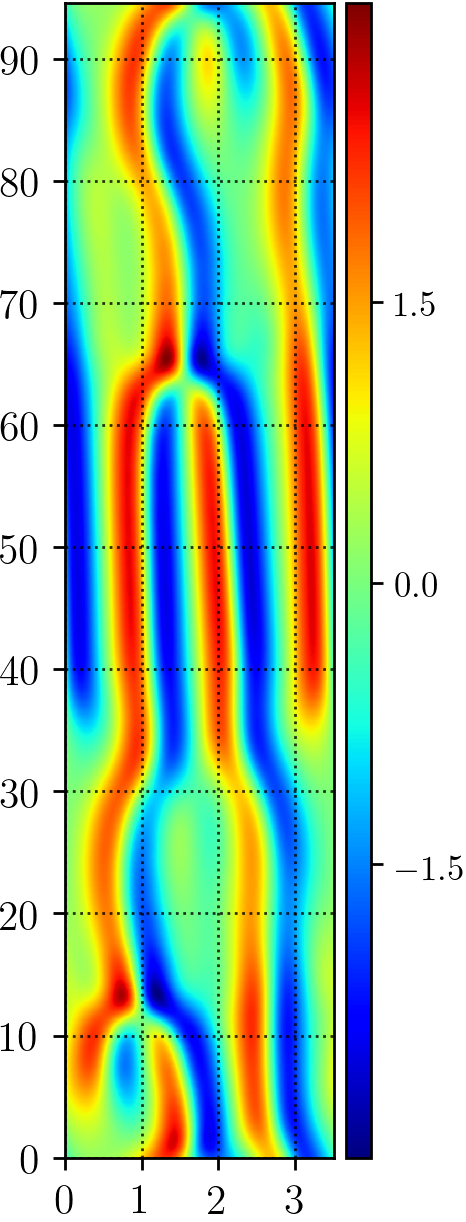
\includegraphics[width=.5\textwidth,height=.5\textheight]{MNG_halfdefect_defect_initial}
\end{minipage}
\begin{minipage}[height=.4\textheight]{.5\textwidth}
\centering \small{\texttt{(b)}}\\
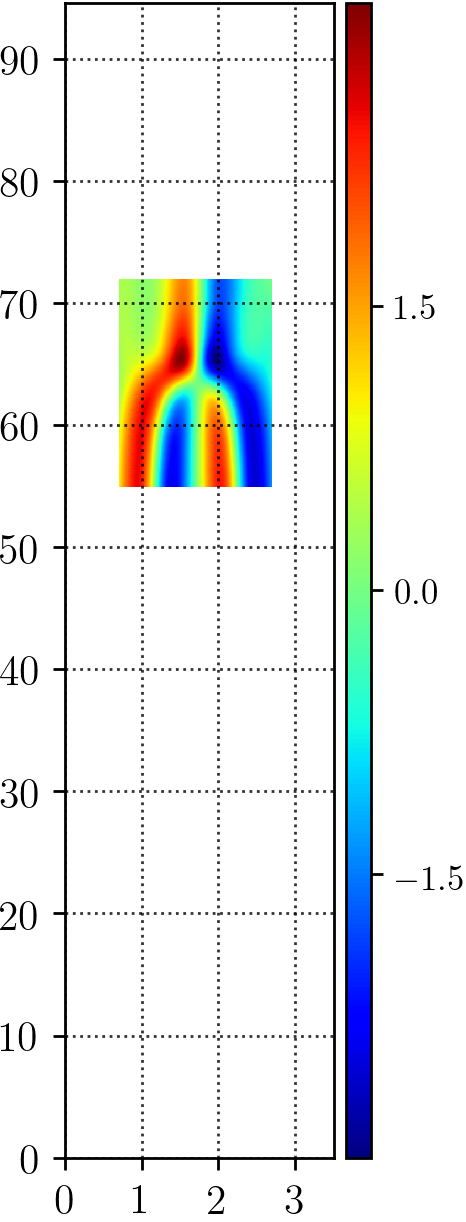
\includegraphics[width=.5\textwidth,height=.5\textheight]{MNG_defect_guess}
\end{minipage}
\begin{minipage}[height=.1\textheight]{\textwidth}
\centering \small{\texttt{(c)}}\\
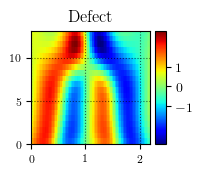
\includegraphics[width=.14\textwidth,height=.1\textheight]{MNG_defect}
\end{minipage}
\caption{ \label{fig:defect}
(a)
$[\speriod{a},\period{a}]=[3.50\cdots,94.59\cdots]$ fundamental domain
of an already computed \twot\ with spatial translation symmetry.
(b)
The clipped-out $[\speriod{b},\period{b}]=[2,17]$ subdomain used the
initial guess for the fundamental domain of a shift-reflect symmetric tile.
(c)
The converged $[\speriod{c},2\period{c}]=[2.07\cdots,18.46\cdots]$ \twot\
with spatial translation symmetry.
}
\end{figure}

\begin{figure}
\begin{minipage}[height=.4\textheight]{.5\textwidth}
\centering \small{\texttt{(a)}}\\
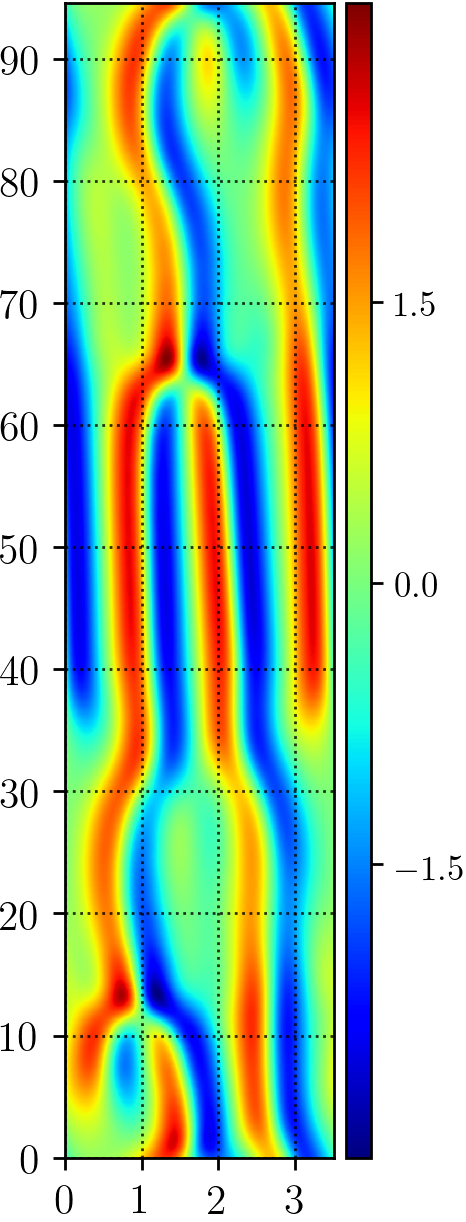
\includegraphics[width=.5\textwidth,height=.5\textheight]{MNG_halfdefect_defect_initial}
\end{minipage}
\begin{minipage}[height=.4\textheight]{.5\textwidth}
\centering \small{\texttt{(b)}}\\
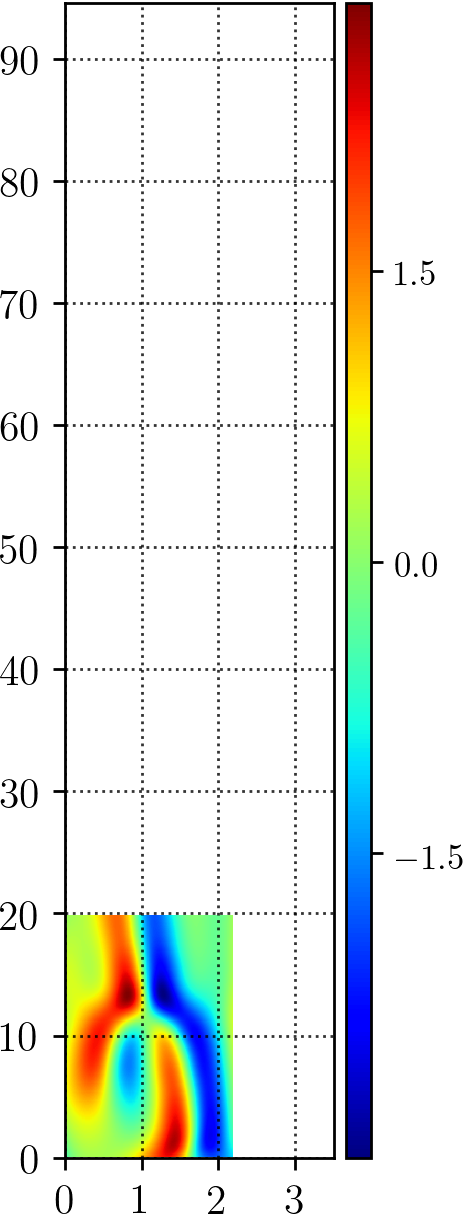
\includegraphics[width=.5\textwidth,height=.5\textheight]{MNG_halfdefect_guess}
\end{minipage}
\begin{minipage}[height=.1\textheight]{\textwidth}
\centering \small{\texttt{(c)}}\\
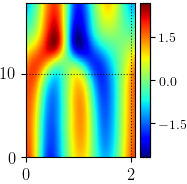
\includegraphics[width=.14\textwidth,height=.12\textheight]{MNG_halfdefect}
\end{minipage}
\caption{ \label{fig:halfdefect}
(a)
$[\speriod{a},\period{a}]=[3.50\cdots,94.59\cdots]$ fundamental domain
of an already computed \twot\ with spatial translation symmetry.
(b)
The clipped-out $[\speriod{b},\period{b}]=[2.2,20]$ subdomain used the
initial guess for the fundamental domain of a shift-reflect symmetric tile.
(c)
The converged $[\speriod{c},2\period{c}]=[2.07\cdots,15.46\cdots]$ \twot\
with spatial translation symmetry.
}
\end{figure}

\begin{figure}
\begin{minipage}[height=.4\textheight]{.5\textwidth}
\centering \small{\texttt{(a)}}\\
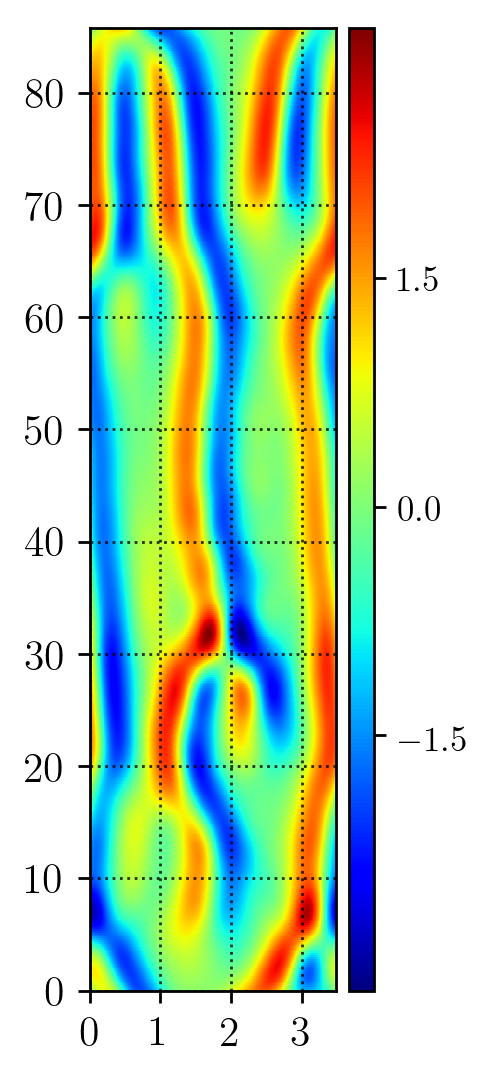
\includegraphics[width=.5\textwidth,height=.5\textheight]{MNG_halfdefect2_initial}
\end{minipage}
\begin{minipage}[height=.4\textheight]{.5\textwidth}
\centering \small{\texttt{(b)}}\\
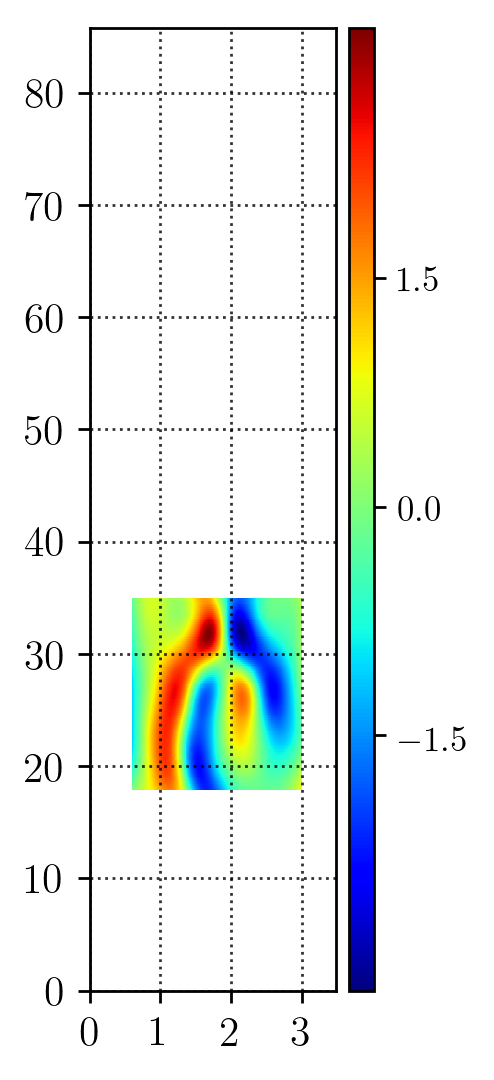
\includegraphics[width=.5\textwidth,height=.5\textheight]{MNG_halfdefect2_guess}
\end{minipage}
\begin{minipage}[height=.1\textheight]{\textwidth}
\centering \small{\texttt{(c)}}\\
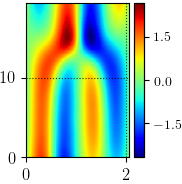
\includegraphics[width=.14\textwidth,height=.1\textheight]{MNG_halfdefect2}
\end{minipage}
\caption{ \label{fig:halfdefect2}
(a)
$[\speriod{a},\period{a}]=[3.50\cdots,85.73\cdots]$ fundamental domain
of an already computed \twot\ with \spt\ shift-reflection symmetry.
(b)
The clipped-out $[\speriod{b},\period{b}]=[2.6,17]$ subdomain used the
initial guess for the fundamental domain of a shift-reflect symmetric tile.
(c)
The converged $[\speriod{c},\period{c}]=[2.06\cdots,19.92\cdots]$ \twot\
with spatial translation symmetry.
}
\end{figure}

\begin{figure}
\begin{minipage}[height=.1\textheight]{.5\textwidth}
\centering \small{\texttt{(a)}}\\
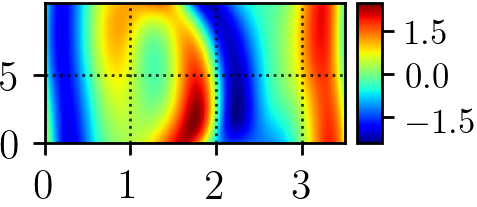
\includegraphics[width=.5\textwidth,height=.1\textheight]{MNG_hook_initial}
\end{minipage}
\begin{minipage}[height=.1\textheight]{.5\textwidth}
\centering \small{\texttt{(b)}}\\
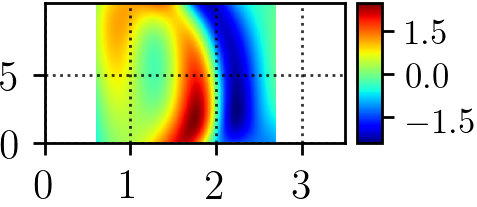
\includegraphics[width=.5\textwidth,height=.1\textheight]{MNG_hook_guess}
\end{minipage}
\begin{minipage}[height=.1\textheight]{\textwidth}
\centering \small{\texttt{(c)}}\\
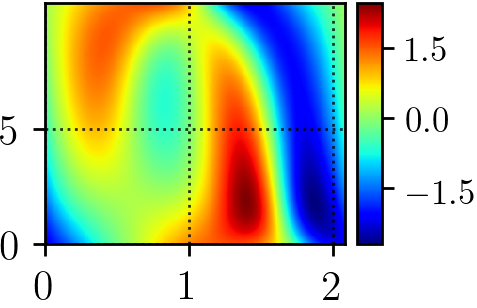
\includegraphics[width=.16\textwidth,height=.1\textheight]{MNG_hook}
\end{minipage}
\caption{ \label{fig:hook}
(a)
$[\speriod{a},\period{a}]=[3.50\cdots,10.25\cdots]$ fundamental domain
of an already computed \twot\ with \spt\ shift-reflection symmetry.
(b)
The clipped-out $[\speriod{b},\period{b}]=[2.1,10.5]$ subdomain used the
initial guess for the fundamental domain of a shift-reflect symmetric tile.
(c)
The converged $[\speriod{c},\period{c}]=[2.08\cdots,9.22\cdots]$  \twot\
with spatial translation symmetry.
}
\end{figure}

\begin{figure}
\begin{minipage}[height=.3\textheight]{.5\textwidth}
\centering \small{\texttt{(a)}}\\
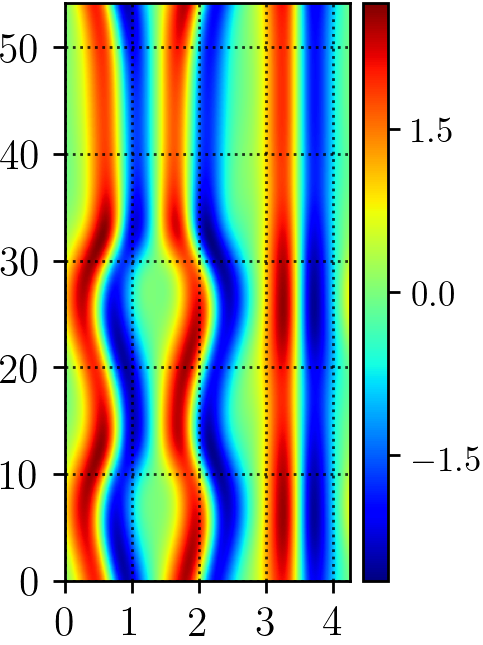
\includegraphics[width=.6\textwidth,height=.4\textheight]{MNG_gap_initial}
\end{minipage}
\begin{minipage}[height=.3\textheight]{.5\textwidth}
\centering \small{\texttt{(b)}}\\
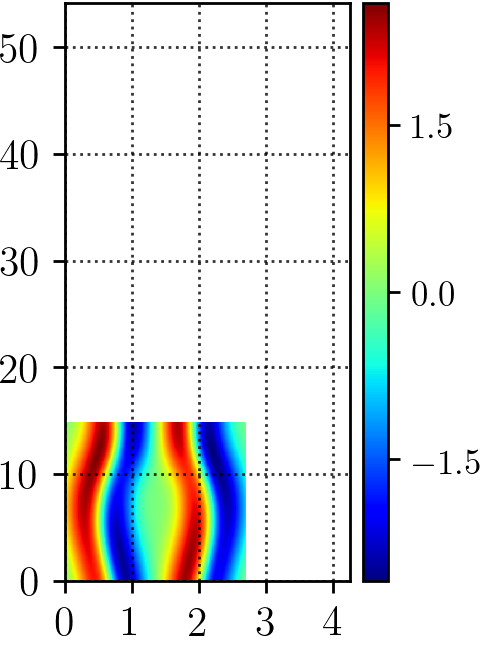
\includegraphics[width=.6\textwidth,height=.4\textheight]{MNG_gap_guess}
\end{minipage}
\begin{minipage}[height=.1\textheight]{\textwidth}
\centering \small{\texttt{(c)}}\\
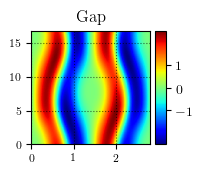
\includegraphics[width=.12\textwidth,height=.13\textheight]{MNG_gap}
\end{minipage}
\caption{ \label{fig:gap}
(a)
$[\speriod{a},\period{a}]=[4.25\cdots,54.13\cdots]$ fundamental domain
of an already computed \twot\ with \spt\ shift-reflection symmetry.
(b)
The clipped-out $[\speriod{b},\period{b}]=[2.7,15]$ subdomain used the
initial guess for the fundamental domain of a shift-reflect symmetric tile.
(c)
The converged $[\speriod{c},\period{c}]=[2.90\cdots,17.95\cdots]$ full
reflection symmetric \twot.
}
\end{figure}


\subsubsection{Sequential subdomain extraction}
While typically robust enough to find tiles in
``one step'',\ie with a single initial condition,
we can also employ our numerical methods iteratively
to find tiles by sequentially converging to
progressively smaller subdomains. We demonstrate
this process in its entirety in \reffig{fig:KStileextraction}; the
result is the same as \reffig{fig:gap} but it is still a good
example.
The advantage of this method is that
by converging progressively smaller \twots\
we increase
our chances of converging to a \spt\ tile.
Numerically, this is because the \twots\
adjust themselves to account for the change in \spt\
domain size and so each succeeding subdomain becomes
a more ``accurate'' initial condition. Note that this
procedure is only applicable if there is a sequence of
subdomains which are approximately doubly periodic;
choosing an arbitrary subdomain would likely fail.
A disadvantage of this method is, of course, that
the repeated computations require more time
and, in our implementation,
the selection of each subdomain is done manually.


\begin{figure}
\begin{minipage}[height=.2\textheight]{.5\textwidth}
\centering \small{\texttt{(a)}}\\
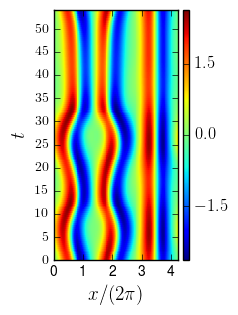
\includegraphics[width=.8\textwidth,height=.5\textheight]{MNGgapzero}
\end{minipage}
\begin{minipage}[height=.2\textheight]{.5\textwidth}
\centering \small{\texttt{(b)}}\\
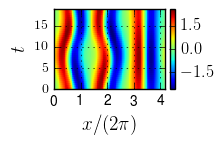
\includegraphics[width=.8\textwidth,height=.18\textheight]{MNGgapone}
\end{minipage}
\begin{minipage}[height=.2\textheight]{.5\textwidth}
\centering \small{\texttt{(c)}}\\
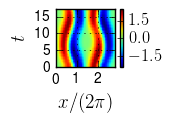
\includegraphics[width=.6\textwidth,height=.18\textheight]{MNGgaptwo}
\end{minipage}
\begin{minipage}[height=.2\textheight]{.48\textwidth}
\centering \small{\texttt{(d)}}\\
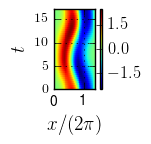
\includegraphics[width=.5\textwidth,height=.18\textheight]{MNGgapthree}
\end{minipage}
\caption{ \label{fig:KStileextraction}
Sequential subdomain extraction to find tiles.
(a) A {\po} from the collection of new solutions
$[\speriod{a},\period{a}]=[4.25\cdots,54.12\cdots]$.
By taking progressively smaller subdomains (b)-(d) and numerically
converging them to \twots\ at each step, we are able to
find the smallest subdomain of (a) which can be converges
to a \twot, namely (d).
(b)$[\speriod{b},\period{b}]=[4.16\cdots,18.93\cdots]$
(c)$[\speriod{c},\period{c}]=[2.79\cdots,17.14\cdots]$
(d)$[\speriod{d},\period{d}]=[1.39\cdots,17.14\cdots]$
}
\end{figure}


\subsubsection{Trinary tile alphabet}
%Describe the most important tiles
As one would expect from ``fundamental'' solutions,
the patterns represented by our
tiles can be described very succinctly.
Typically, each of the tiles contains no more than two
wavelengths as can be seen by the red-blue
(crest-trough) pairs in the corresponding scalar fields.
Because of this we will refer to them by shorthand
names that capture their general behavior and
makes a connection to pattern names which, as we shall see,
are relatively common in the study of fluid flows\rf{MFE04b,W97,JimenezJFM01}.
In the spirit of topological defects\rf{Mermin79,Kleman89,defects07} we
shall give the tiles new names so that they can be easily
identified and referred to.
The first pattern is the single
wavelength equilibrium solution which we shall
refer to as the ``streak'' ((a) from \reffig{fig:tiles}.
The streak tile
is the smallest tile solution, as it has no temporal
dimension because its an \eqv\ solution
but it also has the smallest spatial extent,
$\frac{\speriod{}}{2\pi} \approx 1.02$. As seen
by its near integer value, this spatial extent
happens to be in line with the important spatial
scale of the \KSe\. The streak tile was found
directly as an \eqv\ solution without any extraction efforts.
Although it has no temporal extent, we shall still refer
to this as a \twot\ because the shadowing events \textit{do}
have temporal variations. There seems to be no single time
scale for these shadowing events, but rather the time
scale is determined by the local interactions with its neighbors.
In this way the streak almost plays role as a space filler and
perhaps we should view \spt\ state space as defects inserted into
an infinite \eqv\ solution.

Next we have a tile whose behavior is best
summarized as a two-to-one wavelength merger. Two
wavelengths propagate in time while adjacent spatially;
eventually turning inwards and colliding such that only the
``outer'' pair of remain and form a single wavelength.
%the term defect is too general to refer to a single tile.
We shall refer to this pattern as a ``merger''. This
pattern is strikingly similar to what is know as ``edge
dislocations''\rf{Kleman89} but we prefer to refer to
it as a ``merger'' because in our system this pattern
does not arise as the result of physical strain.
This tile,
((b) \reffig{fig:tiles}), is a \twot\ with dimensions
$\speriod{}\approx 2.07$,$\period{} \approx 18.5$ and
continuous spatial translation symmetry parameter value
approximately equal to a quarter of the domain size
$\sigma \approx 0.2529 \speriod{}$. This tile might
be the most important out of all as we shall see

The last tile consists of a pair
of wavy streaks.
This is exactly how it sounds;
a streak pattern which waves back and forth in
the spatial direction before returning to its
original position.
Not only is it a \twot\ but it is
a \twot\ that lies in the
reflection invariant subspace \refsect{sect:KSsymm},
which allows us to think of the tile in one of
two ways.
We could consider a single wavelength to be the
tile; there are a number of
reasons why we avoid this. Firstly,
sometimes it isn't clear how to distinguish a
single wavy streak from
a regular streak deformed by coupling to its
neighbors. Numerically, these patterns
are so similar that it is possible
to converge to the same solution using either
type of streaks; one would merely increase the
cost functional value as its more ``out of place''
that the other. It might be hard to distinguish between
a single wavy streak and a regular streak, but when you
have a pair of wavy streaks it is quite clear, as
they are symmetry partners which are adjacent to one
another.
Secondly, it seems that the pair of wavy streaks is
shadowed more often, indicating that it is in fact
the representation that we should use.
We will refer to the tile comprised of
two wavy streaks as the
``gap'' tile, because when two wavy streaks
repel each other, it creates a region of spacetime
where the magnitude of the scalar field is
small,\ie, a ``gap'' in the scalar field.
This can be seen in plot (c) of \reffig{fig:KStileextraction}.
The gap tile shown in \reffig{fig:tiles} has dimensions
$\speriod{} \approx 2.81$, $\period{} \approx 17.95$.

%could search for subdomains in \twot\ solutions based on some norm
%between \spt\ rectangles

\begin{figure}
\begin{minipage}[height=.2\textheight]{\textwidth}
\centering \small{\texttt{(a)}}\\
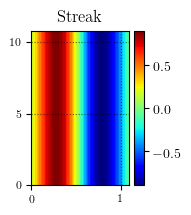
\includegraphics[width=.15\textwidth,height=.1\textheight]{MNG_streak}
\end{minipage}
\begin{minipage}[height=.2\textheight]{.5\textwidth}
\centering \small{\texttt{(b)}}\\
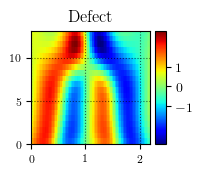
\includegraphics[width=.25\textwidth,height=.1\textheight]{MNG_defect}
\end{minipage}
\begin{minipage}[height=.2\textheight]{.5\textwidth}
\centering \small{\texttt{(c)}}\\
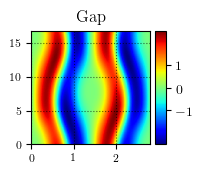
\includegraphics[width=.25\textwidth,height=.1\textheight]{MNG_gap}
\end{minipage}
\caption{ \label{fig:tiles}
(a) The ``streak tile''. Converged \eqv\
$\speriod{s}=1.02\cdots$ demonstrating the fundamental streak
pattern. There
is no temporal variation or scale but the solution $u(x)$ is plotted
as a \spt\ function simply to be consistent with other \spt\ figures.
(b) The ``merger'' tile. Converged \twot\
depicting two-to-one wavelength merging.
This tile is a relative periodic \twot\
$[\speriod{m},\period{m}]=[2.07\cdots,15.86\cdots]$
with spatial shift parameter $\tau_x \approx 1.06$. This
represents a spatial shift approximately equal to a quarter of the domain.
(c) The ``gap'' tile. Converged \twot\
depicting ``wavy streak'' behavior.
$[\speriod{d},\period{d}]=[2.80\cdots,17.14\cdots]$ (plotted in
the full state space for reasons described in \refsect{sect:tiles}).
}
\end{figure}

%After describing which tiles are found, described why they are important.
The merger tile captures a key \spt\ process in a minimal amount
of information. Let us transgress back into
a dynamical systems context to elaborate.
Performing linear stability analysis on the \KSe\ shows
that there is a range of modes which are linearly unstable
\rf{SCD07}.
In addition to this, there exists a mode which is the most unstable
such that the number of wavelengths fluctuates around the most
unstable wavenumber as a function of time.
The number of wavelengths is calculated by
taking the average of the number of
local minima and maxima (which exceed a certain tolerance
value in magnitude to avoid extraneous counting).
The fluctuation of this of quantity indicates that there are
wavelengths being both ``annihilated'' and ``created'' in time.
The merger tile encapsulates both of these processes.
Previously, we described
the merger tile as being a two to one wavelength merger;
this is the ``annihilation'' process in action. There's slightly more
to the story, however, as very shortly after the wavelength merger a
new wavelength is born in the vacant space. This can
be seen in the depiction of the converged merger tile (c) from
\reffig{fig:defect}.
These three tiles provide us with an entirely new
perspective of how to view the \KSe, which is that the
\spt\ behavior of solutions seems to be described by
the interaction of crest-trough pairs.
Specifically, the streak tile describes
how wavelengths remain constant in time,
the gap tile describes how wavelengths repel each other
and the merger tile captures how wavelengths attract
and combine. Technically,
on a small \spt\ domain the gap tile can be interpreted as
both attracting and repelling because the domain is periodic.
Therefore, an alternative description of the gap tile is
that it represents wavelength attraction without the
wavelength merger.
This emergent behavior seems to be unique to the \spt\
formulation or is at least
not obvious by inspection of the \KSe\ \refeq{e-ks} alone.

The largest concern regarding this formulation is
whether or not our alphabet is missing a tile.
This would likely be devastating as we know from
the work on cycle expansions that short cycles has the greatest
importance\rf{Christiansen97}.
The only evidence we have to indicate that we have
found all tiles is that we simply have not found any more unique
tiles despite a thorough search.
Most trials converge to known tiles (up to symmetry operations).
This can be seen in the comparison between converged \twots\ in
\reffig{fig:tilerepeats}.

\begin{figure}
\begin{minipage}[height=.2\textheight]{.5\textwidth}
\centering \small{\texttt{(a)}}\\
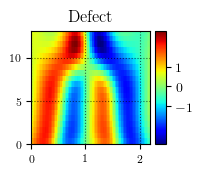
\includegraphics[width=.3\textwidth,height=.1\textheight]{MNG_defect}
\end{minipage}
\begin{minipage}[height=.2\textheight]{.5\textwidth}
\centering \small{\texttt{(b)}}\\
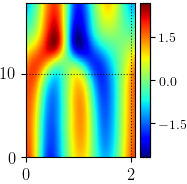
\includegraphics[width=.3\textwidth,height=.1\textheight]{MNG_halfdefect}
\end{minipage}
\begin{minipage}[height=.2\textheight]{.5\textwidth}
\centering \small{\texttt{(c)}}\\
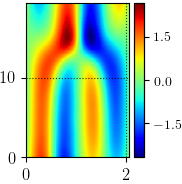
\includegraphics[width=.3\textwidth,height=.1\textheight]{MNG_halfdefect2}
\end{minipage}
\begin{minipage}[height=.2\textheight]{.5\textwidth}
\centering \small{\texttt{(d)}}\\
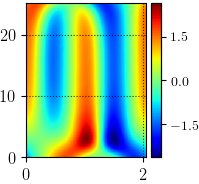
\includegraphics[width=.3\textwidth,height=.1\textheight]{MNG_hookcont}
\end{minipage}
\caption{ \label{fig:tilerepeats}
(a) \twoT\ from \reffig{fig:defect}(c), $[\speriod{a},2\period{a}]=[2.07\cdots,18.46\cdots]$ \twot\
with spatial translation symmetry.
(b) \twoT\ from \reffig{fig:halfdefect}(c), $[\speriod{c},2\period{c}]=[2.07\cdots,15.46\cdots]$ \twot\
with spatial translation symmetry.
(c) \twoT\ from \reffig{fig:halfdefect2}(c), $[\speriod{c},\period{c}]=[2.06\cdots,19.92\cdots]$ \twot\
with spatial translation symmetry.
(d)\twoT\ resulting from performing pseudo-arclength continuation
on \reffig{fig:hook}(c). Final \twot\ has $[\speriod{c},\period{c}]=[2.06\cdots,23.21\cdots]$
and spatial translation symmetry.
}
\end{figure}

There are also examples which do not converge to tiles but to
combinations of tiles. Examples include \reffig{fig:hookondefect},
\reffig{fig:hookondefect2},\reffig{fig:hookondefect3}. These attempts
all started with what appears to be two patterns conjoined in time.
One might ask why we chose these as tile candidates given
they have more than one constituent pattern; our reason is that
they were frequently shadowed and we did not know \textit{a priori} what
tiles existed, hence their consideration as tile candidates.
Their respective converged \twots\ all
appear to be two (symmetry related) copies of the
merger tile conjoined temporally, indicating that the initial conditions
were indeed two separate patterns conjoined in time. As just mentioned,
in the converged \twots\ the two conjoined patterns are much more similar
that in the initial conditions. The explanation for this process can be explained
by the discovery that tiles do not exist as stand alone solutions; rather, they
exist in continuous families (related by smooth deformations) parameterized by
\spt\ domain size parameters $\speriod{}$ and $\period{}$.

\begin{figure}
\begin{minipage}[height=.4\textheight]{.5\textwidth}
\centering \small{\texttt{(a)}}\\
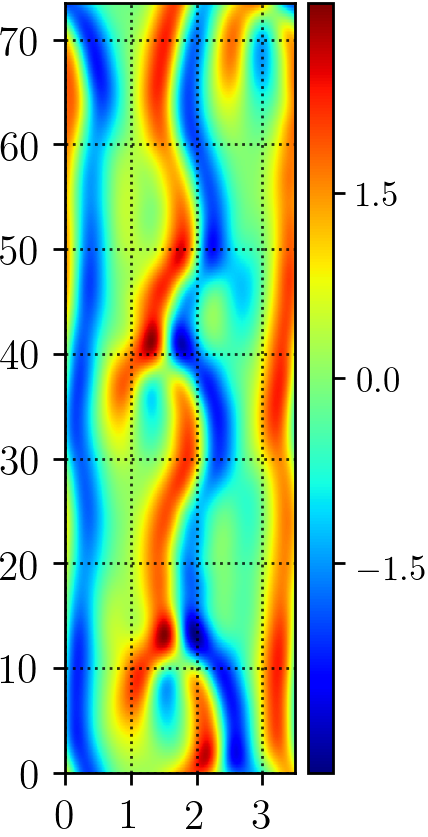
\includegraphics[width=.5\textwidth,height=.4\textheight]{MNG_hookondefect_initial}
\end{minipage}
\begin{minipage}[height=.4\textheight]{.5\textwidth}
\centering \small{\texttt{(b)}}\\
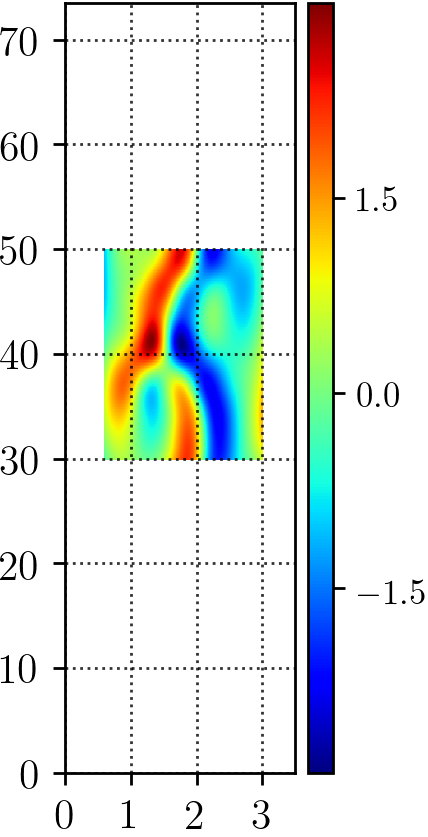
\includegraphics[width=.5\textwidth,height=.4\textheight]{MNG_hookondefect_guess}
\end{minipage}
\begin{minipage}[height=.4\textheight]{\textwidth}
\centering \small{\texttt{(c)}}\\
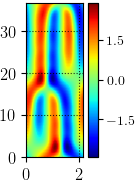
\includegraphics[width=.2\textwidth,height=.22\textheight]{MNG_hookondefect}
\end{minipage}
\caption{ \label{fig:hookondefect}
(a)
$[\speriod{a},\period{a}]=[3.49\cdots,73.52\cdots]$ fundamental domain
of an already computed \twot\ with \spt\ shift-reflection symmetry.
(b)
The clipped-out $[\speriod{b},\period{b}]=[2.4,20]$ subdomain used the
initial guess for the fundamental domain of a shift-reflect symmetric tile.
(c)
The converged $[\speriod{c},\period{c}]=[2.09\cdots,52.00\cdots]$ full
shift-reflect symmetric \twot.
}
\end{figure}

\begin{figure}
\begin{minipage}[height=.4\textheight]{.5\textwidth}
\centering \small{\texttt{(a)}}\\
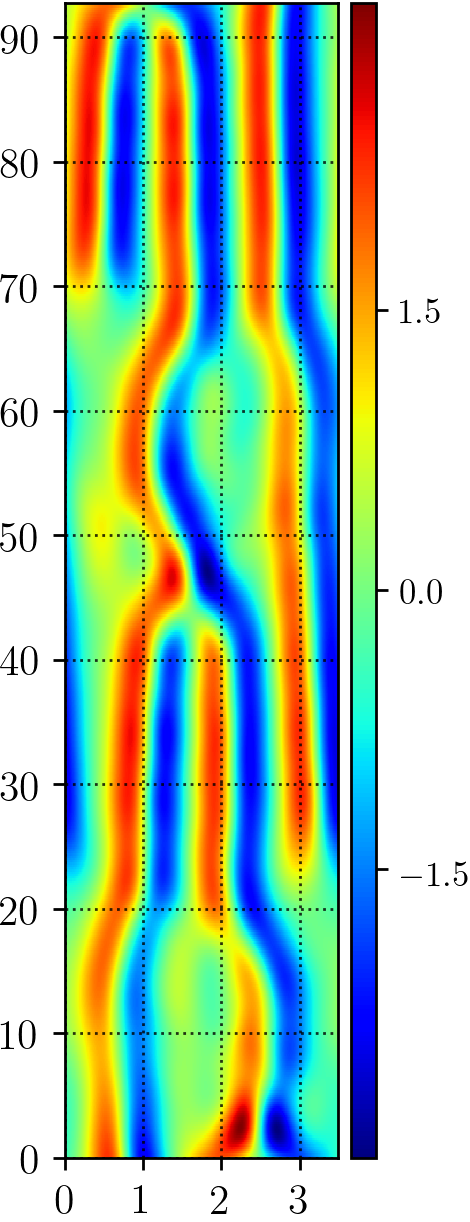
\includegraphics[width=.5\textwidth,height=.5\textheight]{MNG_hookondefect2_initial}
\end{minipage}
\begin{minipage}[height=.4\textheight]{.5\textwidth}
\centering \small{\texttt{(b)}}\\
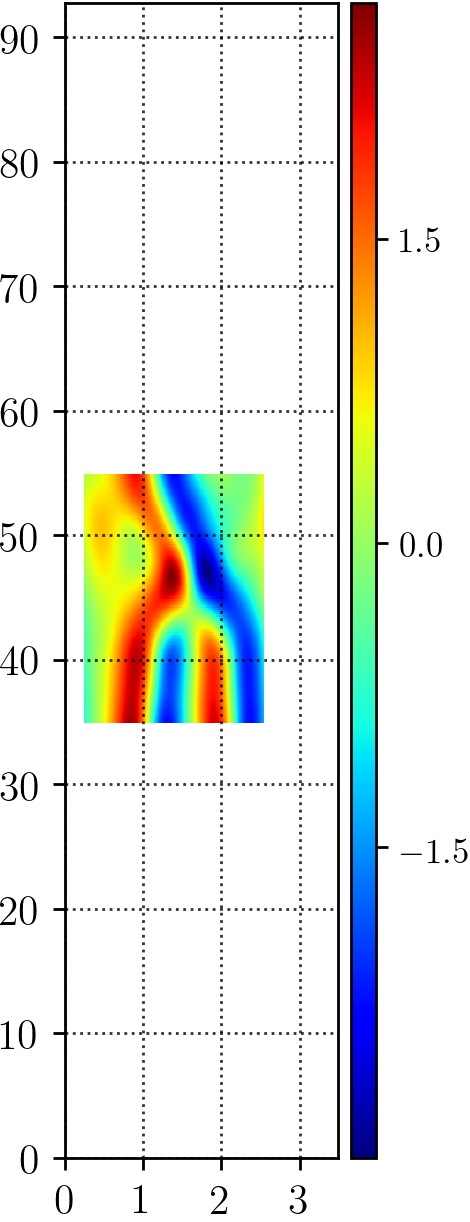
\includegraphics[width=.5\textwidth,height=.5\textheight]{MNG_hookondefect2_guess}
\end{minipage}
\begin{minipage}[height=.1\textheight]{\textwidth}
\centering \small{\texttt{(c)}}\\
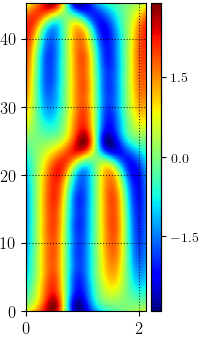
\includegraphics[width=.2\textwidth,height=.22\textheight]{MNG_hookondefect2}
\end{minipage}
\caption{ \label{fig:hookondefect2}
(a)
$[\speriod{g},\period{g}]=[3.49\cdots,92.77\cdots]$ fundamental domain
of an already computed \twot\ with \spt\ shift-reflection symmetry.
(b)
The clipped-out $[\speriod{g},\period{g}]=[2.3,20]$ subdomain used the
initial guess for the fundamental domain of a shift-reflect symmetric tile.
(c)
The converged $[\speriod{g},\period{g}]=[2.12\cdots,45.25\cdots]$ full
shift-reflect symmetric \twot.
}
\end{figure}

\begin{figure}
\begin{minipage}[height=.4\textheight]{.32\textwidth}
\centering
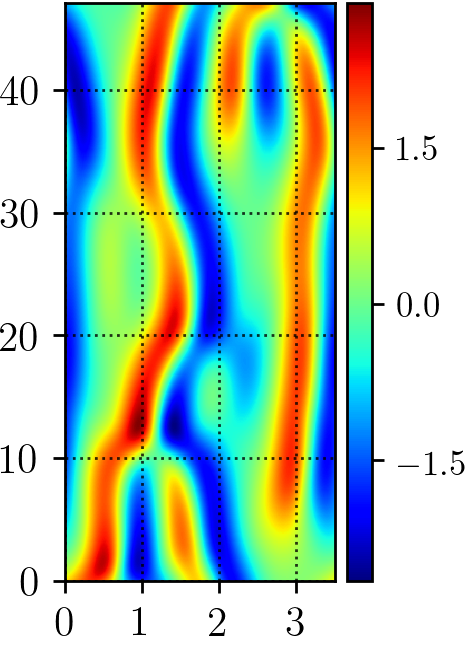
\includegraphics[width=.9\textwidth,height=.23\textheight]{MNG_hookondefect3_initial}
   \\ \small{\texttt{(a)}}
\end{minipage}
\begin{minipage}[height=.4\textheight]{.32\textwidth}
\centering
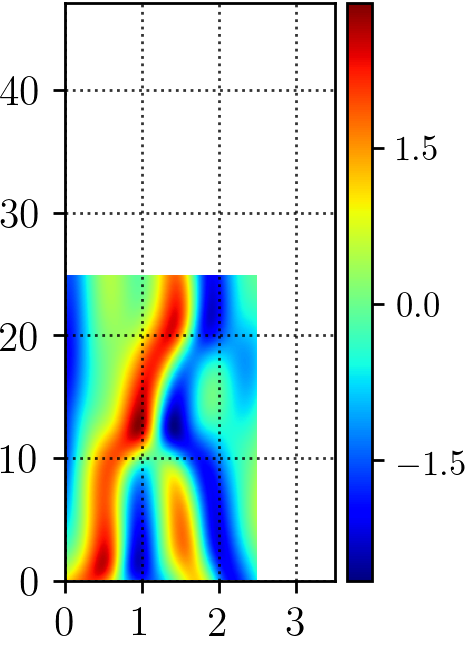
\includegraphics[width=.9\textwidth,height=.23\textheight]{MNG_hookondefect3_guess}
   \\ \small{\texttt{(b)}}
\end{minipage}
\begin{minipage}[height=.4\textheight]{.32\textwidth}
\centering
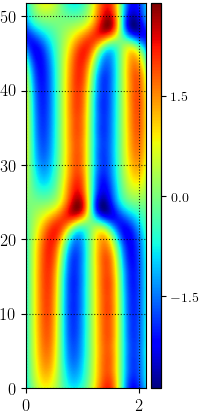
\includegraphics[width=0.5\textwidth,height=.25\textheight]{MNG_hookondefect3}
   \\ \small{\texttt{(c)}}
\end{minipage}
\caption{ \label{fig:hookondefect3}
(a)
$[\speriod{0},\period{0}]=[3.49\cdots,47.77\cdots]$ fundamental domain
of an already computed \twot\ with \spt\ shift-reflection symmetry.
(b)
The clipped-out $[\speriod{g},\period{g}]=[2.06,25]$ subdomain used the
initial guess for the fundamental domain of a shift-reflect symmetric tile.
(c)
The converged $[\speriod{p},2\period{p}]=[2.12\cdots,51.73\cdots]$ full
shift-reflect symmetric \twot.
}
\end{figure}

    \PC{2019-09-20}{
Length units (ticks on \ssp-axis) in \reffig{fig:hookondefect3} (vs. the
numbers stated in the caption) seem screwy, they should be in units of
$\tildeL = \speriod{}/2\pi$, or (but I do not think that would be good)
in ``mean wavelength'' units $2\pi\sqrt{2}$, see \reffig{f:ks_largeL}. Or
are you plotting lengths in $\speriod{}$ units?
    }
    \PC{2019-05-16}{
Perhaps replace spatial period everywhere with $\tildeL=\speriod{}/2\pi$
, define \tildeL\ with a numbered equation early on. Than have to do it
for the time $\period{}/2\pi$ as well...?
    }


\subsubsection{Continuous families of tiles}
The streak, gap, and merger tiles
will be used to construct known and new
solutions. This of course supports our claim that \twots\ and tiles
are shadowing partners. Tiles are never exhibited exactly
in \twots, however, because of \spt\ coupling.
Another way of phrasing this is that the shadowed tiles
deform in order to fit on a \spt\ domain and obey the \KSe\
simultaneously. This deformation makes it hard to quantify
the shadowing process as we lack a good metric. This
coupling also creates difficulties and raises
questions when combining tiles to form
initial conditions as we shall see in \refsect{sect:glue}.
Through some investigation it seems that
these ``deformations'' are in fact
various instances of continuous
families. This can be shown to by applying pseudo-arclength continuation
of the tiles with respect to the parameters $T,L$.
%Describe that the three tiles actually exist in continuous families.
%Describe the continuous families themselves.
One such related pair of tiles
that appear different but are in fact representations
of the same pattern are the converged \twots\ from \reffig{fig:defect}
and \reffig{fig:hook}. Their comparison by numerical continuation
is shown in \reffig{fig:tilerepeats}, along with other similar
patterns.
In summary, the comparison of \reffig{fig:tilerepeats}
demonstrates that the tiles appear identical up to translational
symmetries; we could fix the phases of the \spt\ \Fcs\
to demonstrate their equality but we would rather stress that
the same tile can be represented in numerous ways. Not
only is there a continuous family parameterized by
the \spt\ area, but also for each \spt\ area there
is a group orbit (states reachable by symmetry operations)
resulting from continuous and discrete symmetries.
The comparison of \reffig{fig:defect}
and \reffig{fig:hook} we have demonstrated allows us
to reinterpret the results from
\reffig{fig:hookondefect},
\reffig{fig:hookondefect2},\reffig{fig:hookondefect3}.
This new interpretation is that the initial conditions shadow
the same tile \textit{family} twice; not the same exact tile twice.
Upon hindsight this actually makes a lot of sense as no shadowing events
are ever identical.
Perhaps this should have been obvious from the start
because larger \twots\ also
exist in continuous families, but the reverse idea might
be more enlightening.
For instance, it might be more correct to say that \twots\
exist in continuous families \textit{because} the tiles exist
in continuous families, not the other way around.
This interpretation
seems to have more impact but it
is not without bias as it supports our tiling
methods, however,
showing that \twots\ can be constructed from
specific tile combinations
provides some good evidence.
%Describe the impact of having continuous families and its meaning.
To account for continuous families of tiles we must
adjust our description of our \spt\ symbolic dynamics.
The two-dimensional symbolic blocks (one dimension for each continuous
symmetry) now consist of ``lattice sites''  which are not of the conventional
discrete type but rather each site will represent a \twot\ solution defined
on a malleable \spt\ domain parameterized by $\period{}$,$\speriod{}$,$\sigma$.
This is perhaps what we should have expected to begin with, as the deformability
aligns itself with the principle of shadowing. The shadowing of \spt\ \twots\
can be described by regions of spacetime that are ``close'' to the \twot\ in some norm.
The explanation for why these shadowing events
appear as one family member over another
is quantitatively hard to describe but
qualitatively the \twot\ must be
coupled to its \spt\ neighbors in order to locally solve the \KSe, so
whichever family member fits on the domain with its neighbors is the
one that is realized.
The numerical continuation performed in \reffig{fig:defectfamily} demonstrates
at the very least that the merger tile can exist on multiple \spt\ domain sizes.
It does not exist on all domain sizes, however; the displayed examples are close
to the ``boundaries'' of the continuous family (with respect to $\speriod{}$).
When the solutions (a) and (c) are numerically to smaller (larger) $\speriod{}$
they approach a homoclinic connection and \reqv\ solutions, respectively.
We expect that the discovery of continuous
families actually helps us immensely.
The benefit is that it provides a much needed
flexibility towards finding admissible patterns.
In summary, an optimistic interpretation
is that we have a ternary alphabet for our
symbolic dynamics parameterized by parameters
such as $L$ and $T$.
This dramatic reduction in the number of available patterns (seemingly
innumerable down to three, give or take an infinite number
of continuous deformations) seems too good to be true.
As we shall see, however, this trinary
alphabet is indeed sufficient to reproduce
known solutions and produce new solutions
which provides empirical evidence
that shows we are on the right track.
In fact, with some manual labor, we
were able to produce an initial condition that
converged to the known solution. This is demonstrated
in \reffig{fig:trinarytiling}.
The explicit construction of the
initial condition used in \reffig{fig:trinarytiling}
is given by \reffig{fig:tilingschematic}.


\begin{figure}
\begin{minipage}[height=.2\textheight]{.3\textwidth}
\centering \small{\texttt{(a)}}\\
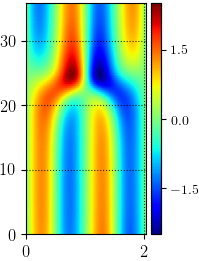
\includegraphics[width=.5\textwidth,height=.18\textheight]{MNGdefectsmallL}
\end{minipage}
\begin{minipage}[height=.2\textheight]{.3\textwidth}
\centering \small{\texttt{(b)}}\\
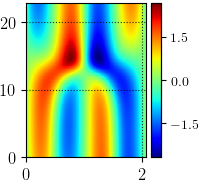
\includegraphics[width=.5\textwidth,height=.14\textheight]{MNGdefectmediumL}
\end{minipage}
\begin{minipage}[height=.2\textheight]{.3\textwidth}
\centering \small{\texttt{(c)}}\\
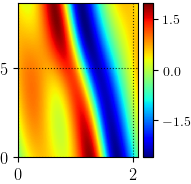
\includegraphics[width=.5\textwidth,height=.07\textheight]{MNGdefectlargeL}
\end{minipage}
\caption{ \label{fig:defectfamily}
Demonstration of the continuous merger tile family via numerical continuation.
The family exists approximately on the range of domain sizes $\frac{L}{2\pi} \in
[\approx 2, \approx 2.13]$. \twoT\ solutions reached by numerical continuation
of the merger tile solution with \spt\ dimensions,
(a) $[\speriod{a},\period{a}]=[2.03\cdots,35.73\cdots]$,
(b) $[\speriod{b},\period{b}]=[2.06\cdots,22.80\cdots]$,
(b) $[\speriod{c},\period{c}]=[2.08\cdots,8.61\cdots]$
}
\end{figure}

\subsubsection{\twoTs\ from tiles}
\begin{figure}
\begin{minipage}[height=.4\textheight]{.5\textwidth}
\centering \small{\texttt{(a)}}\\
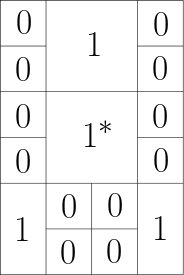
\includegraphics[width=.5\textwidth,height=.25\textheight]{MNG_symbolicblock}
\end{minipage}
\begin{minipage}[height=.4\textheight]{.5\textwidth}
\centering \small{\texttt{(b)}}\\
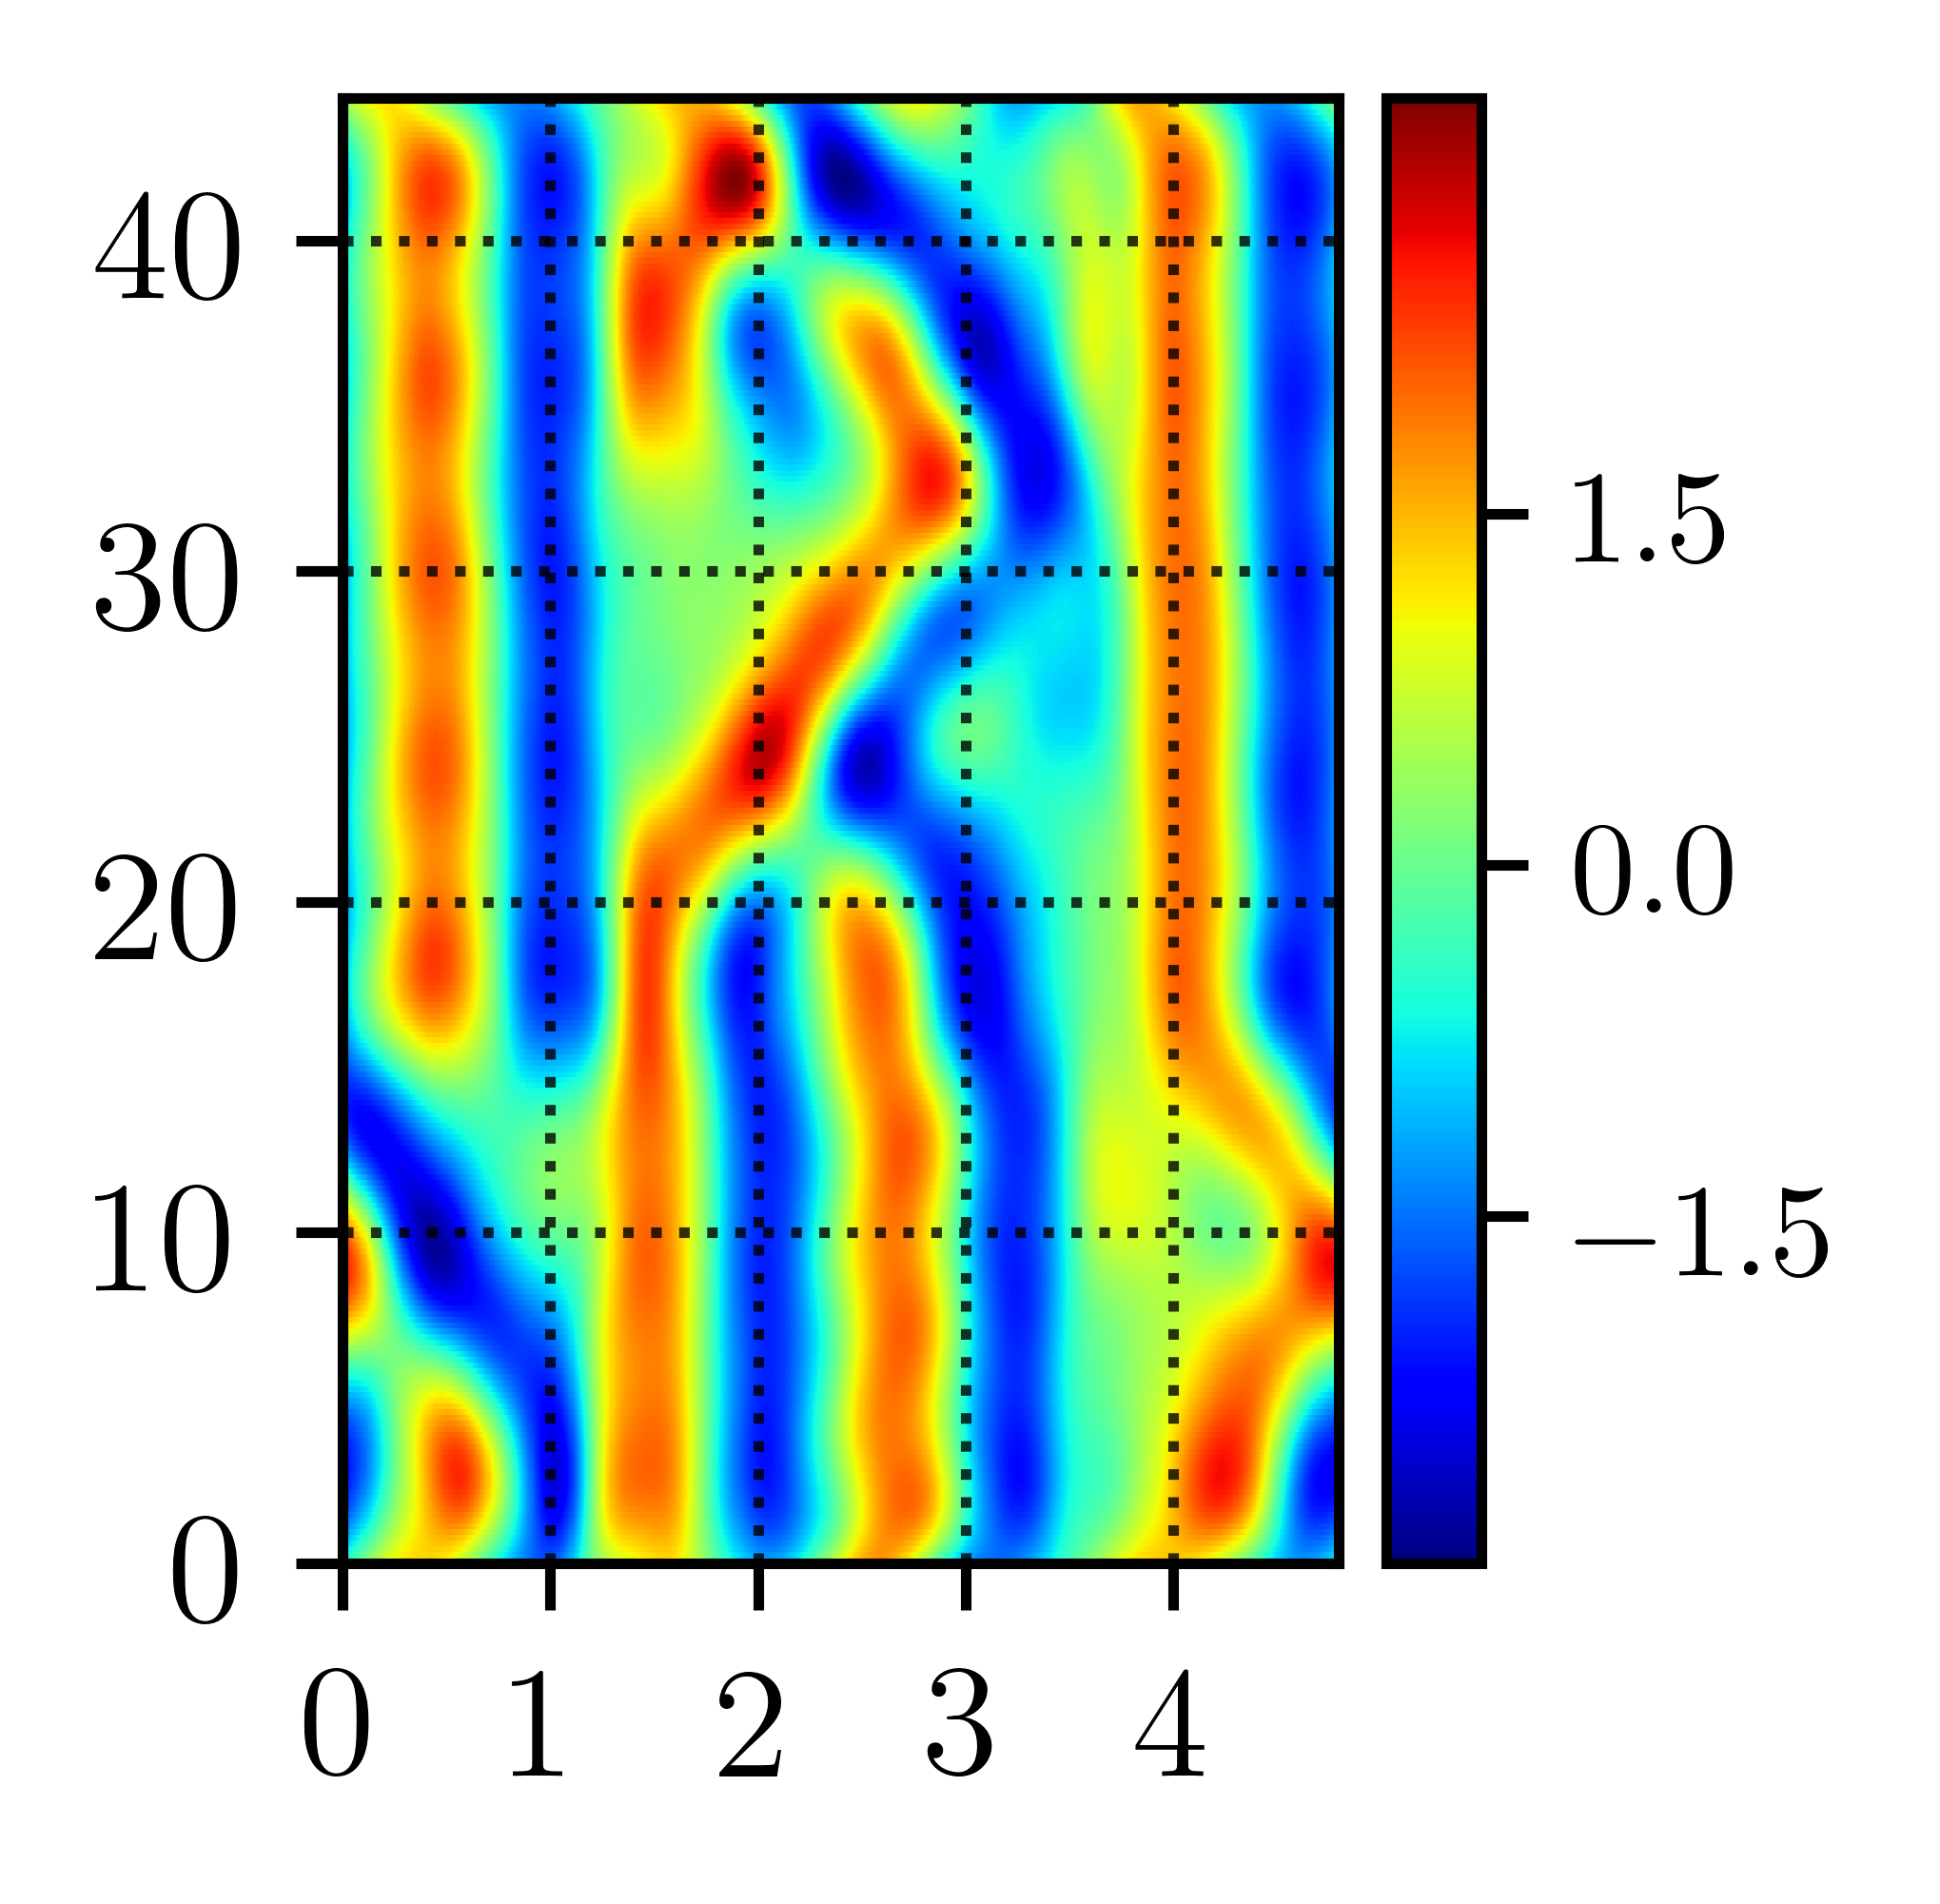
\includegraphics[width=.7\textwidth,height=.32\textheight]{MNG_trinary_initial}
\end{minipage}
\begin{minipage}[height=.4\textheight]{.5\textwidth}
\centering \small{\texttt{(c)}}\\
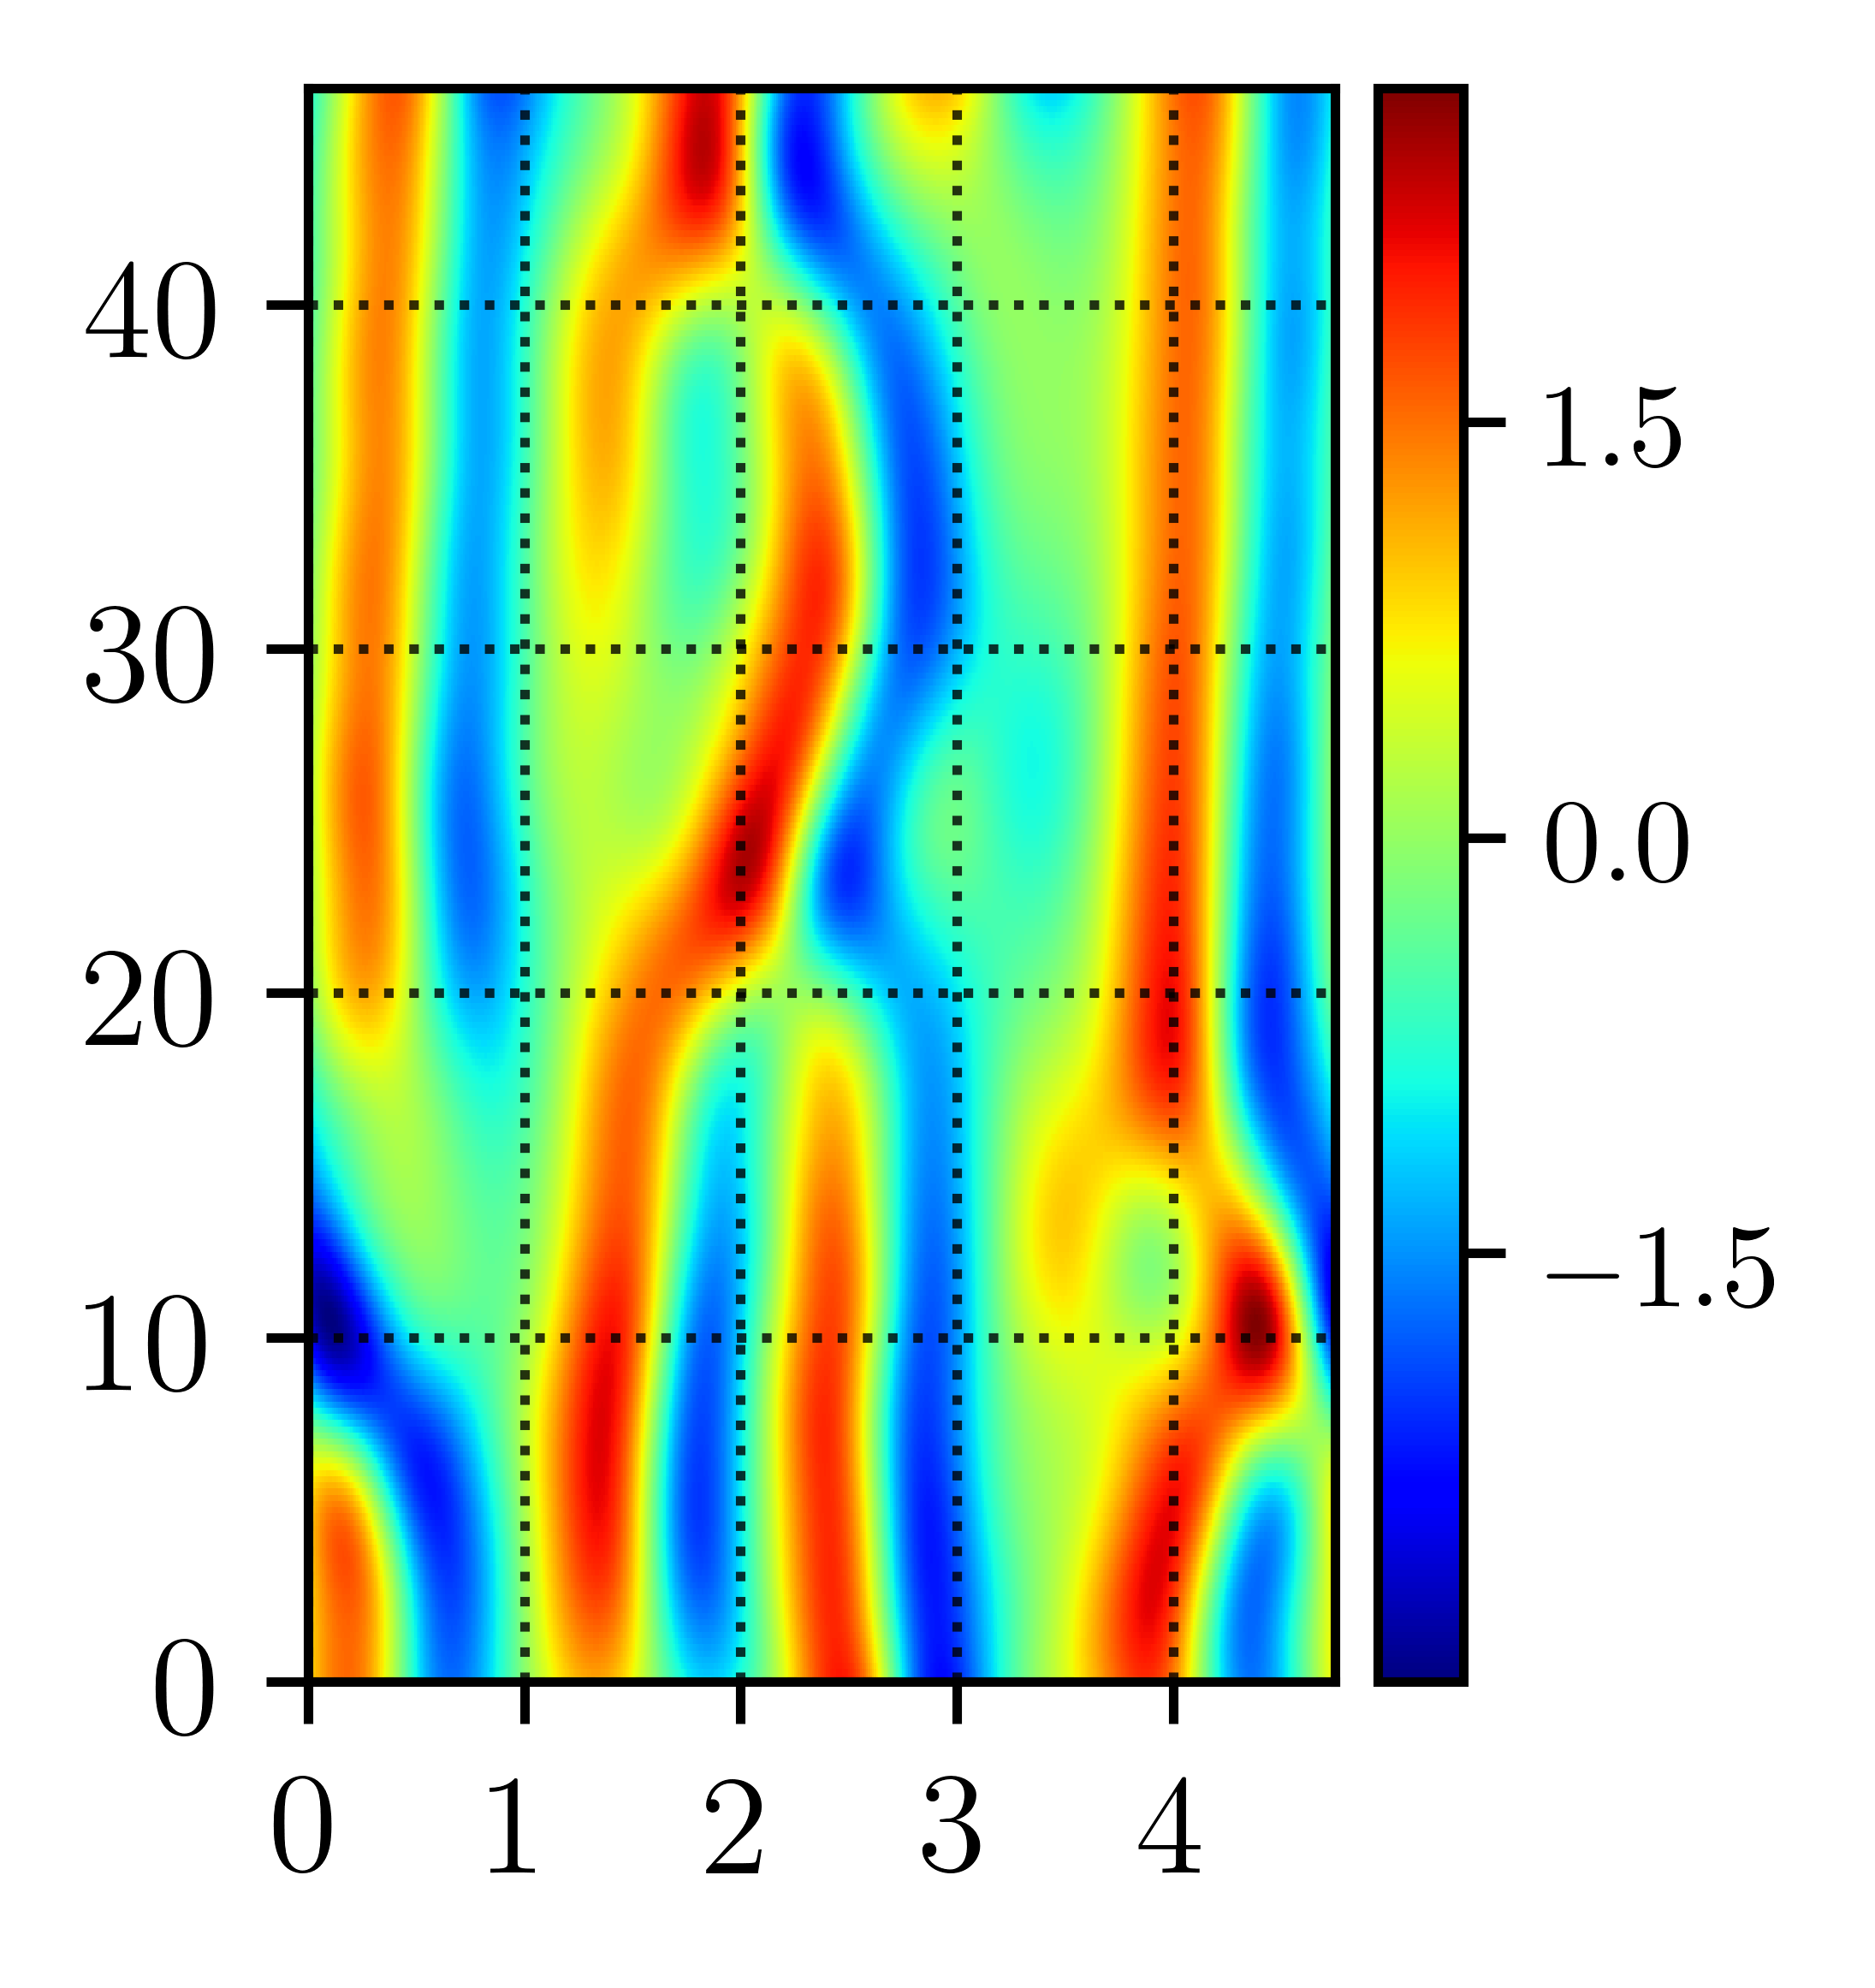
\includegraphics[width=.7\textwidth,height=.32\textheight]{MNG_trinary_final}
\end{minipage}
\begin{minipage}[height=.4\textheight]{.5\textwidth}
\centering \small{\texttt{(d)}}\\
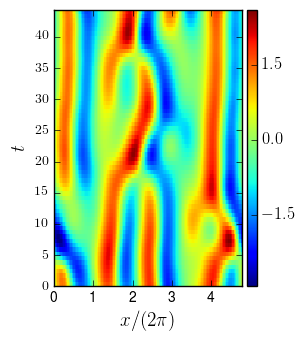
\includegraphics[width=.7\textwidth,height=.32\textheight]{MNG_ppo_L30_T44}
\end{minipage}
\caption{ \label{fig:trinarytiling}
(a) \Spt\ symbolic block representation created using group orbits
of three tile families,
(b) initial condition produced by combining tiles according to (a);
dimensions initialized at $[\speriod{b},\period{b}]=[4.79\cdots,88.62\cdots]$,
(c) converged \twot\ when using (b) as an initial condition,
(d) targeted \twot\ which (c) was trying to match.
}
\end{figure}


\begin{figure}
\begin{minipage}[height=.05\textheight]{.3\textwidth}
\centering \small{\texttt{(a)}}\\
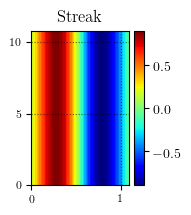
\includegraphics[width=.3\textwidth,height=.1\textheight]{MNG_streak}
\end{minipage}
\begin{minipage}[height=.05\textheight]{.3\textwidth}
\centering \small{\texttt{(b)}}\\
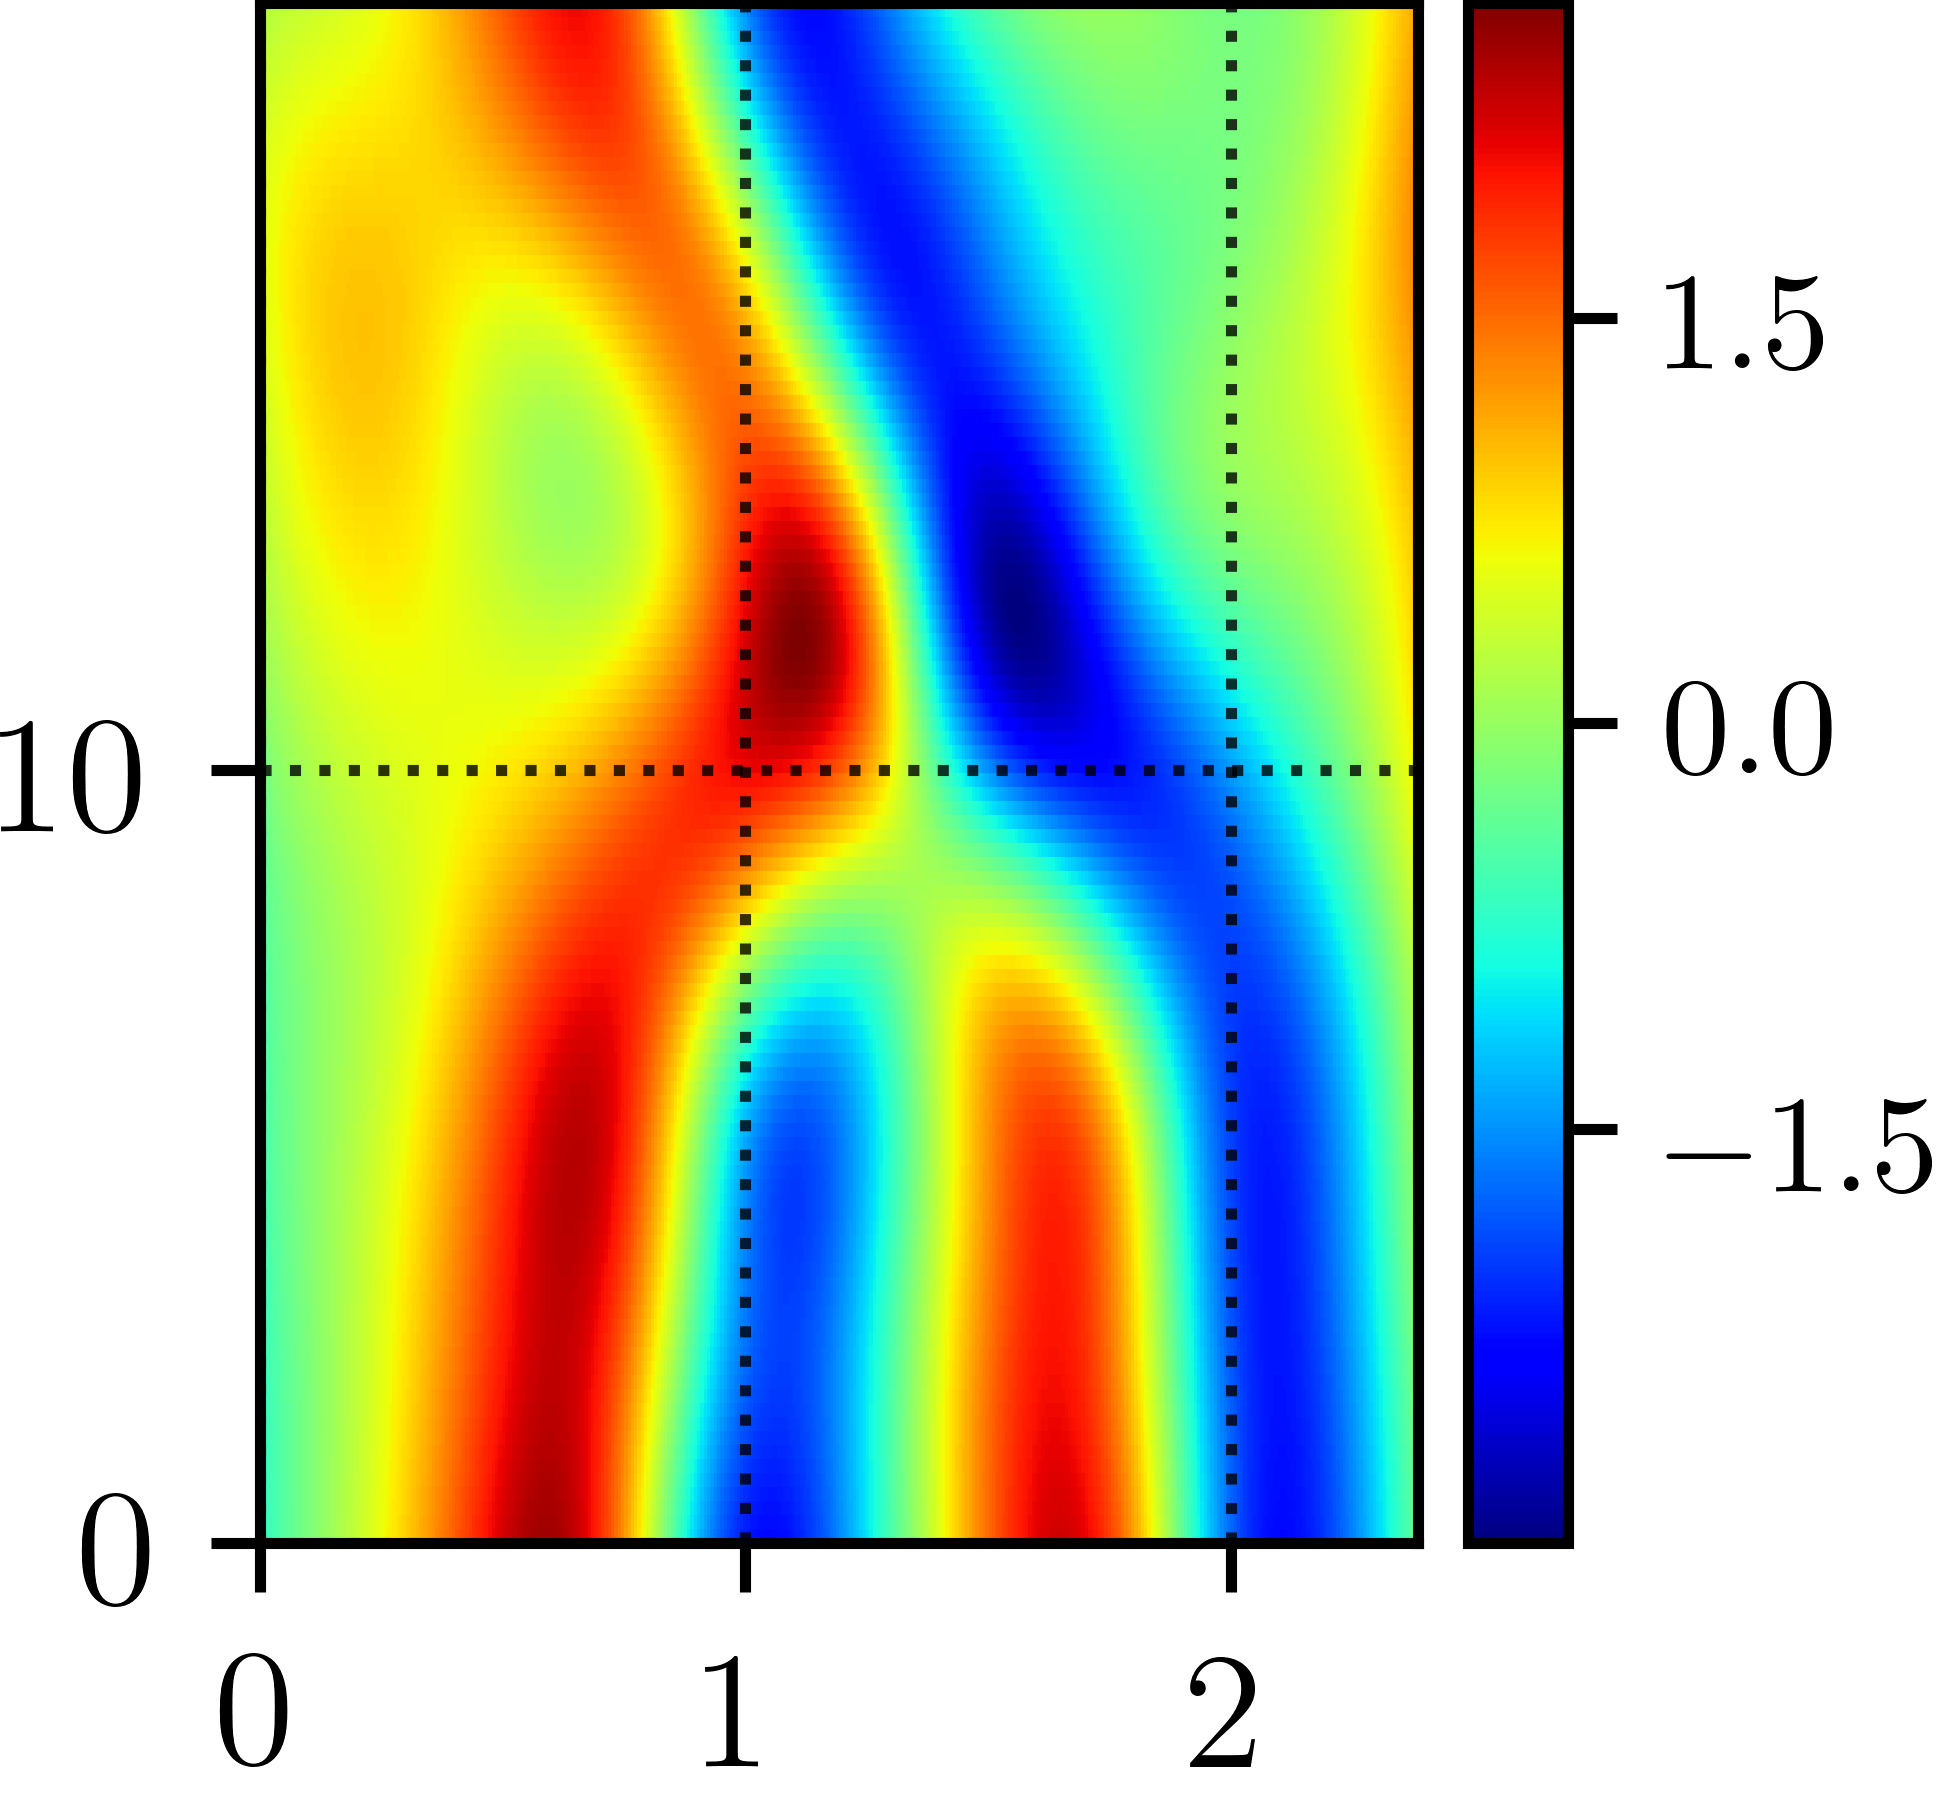
\includegraphics[width=.4\textwidth,height=.1\textheight]{MNG_hookondefecterg}
\end{minipage}
\begin{minipage}[height=.05\textheight]{.3\textwidth}
\centering \small{\texttt{(c)}}\\
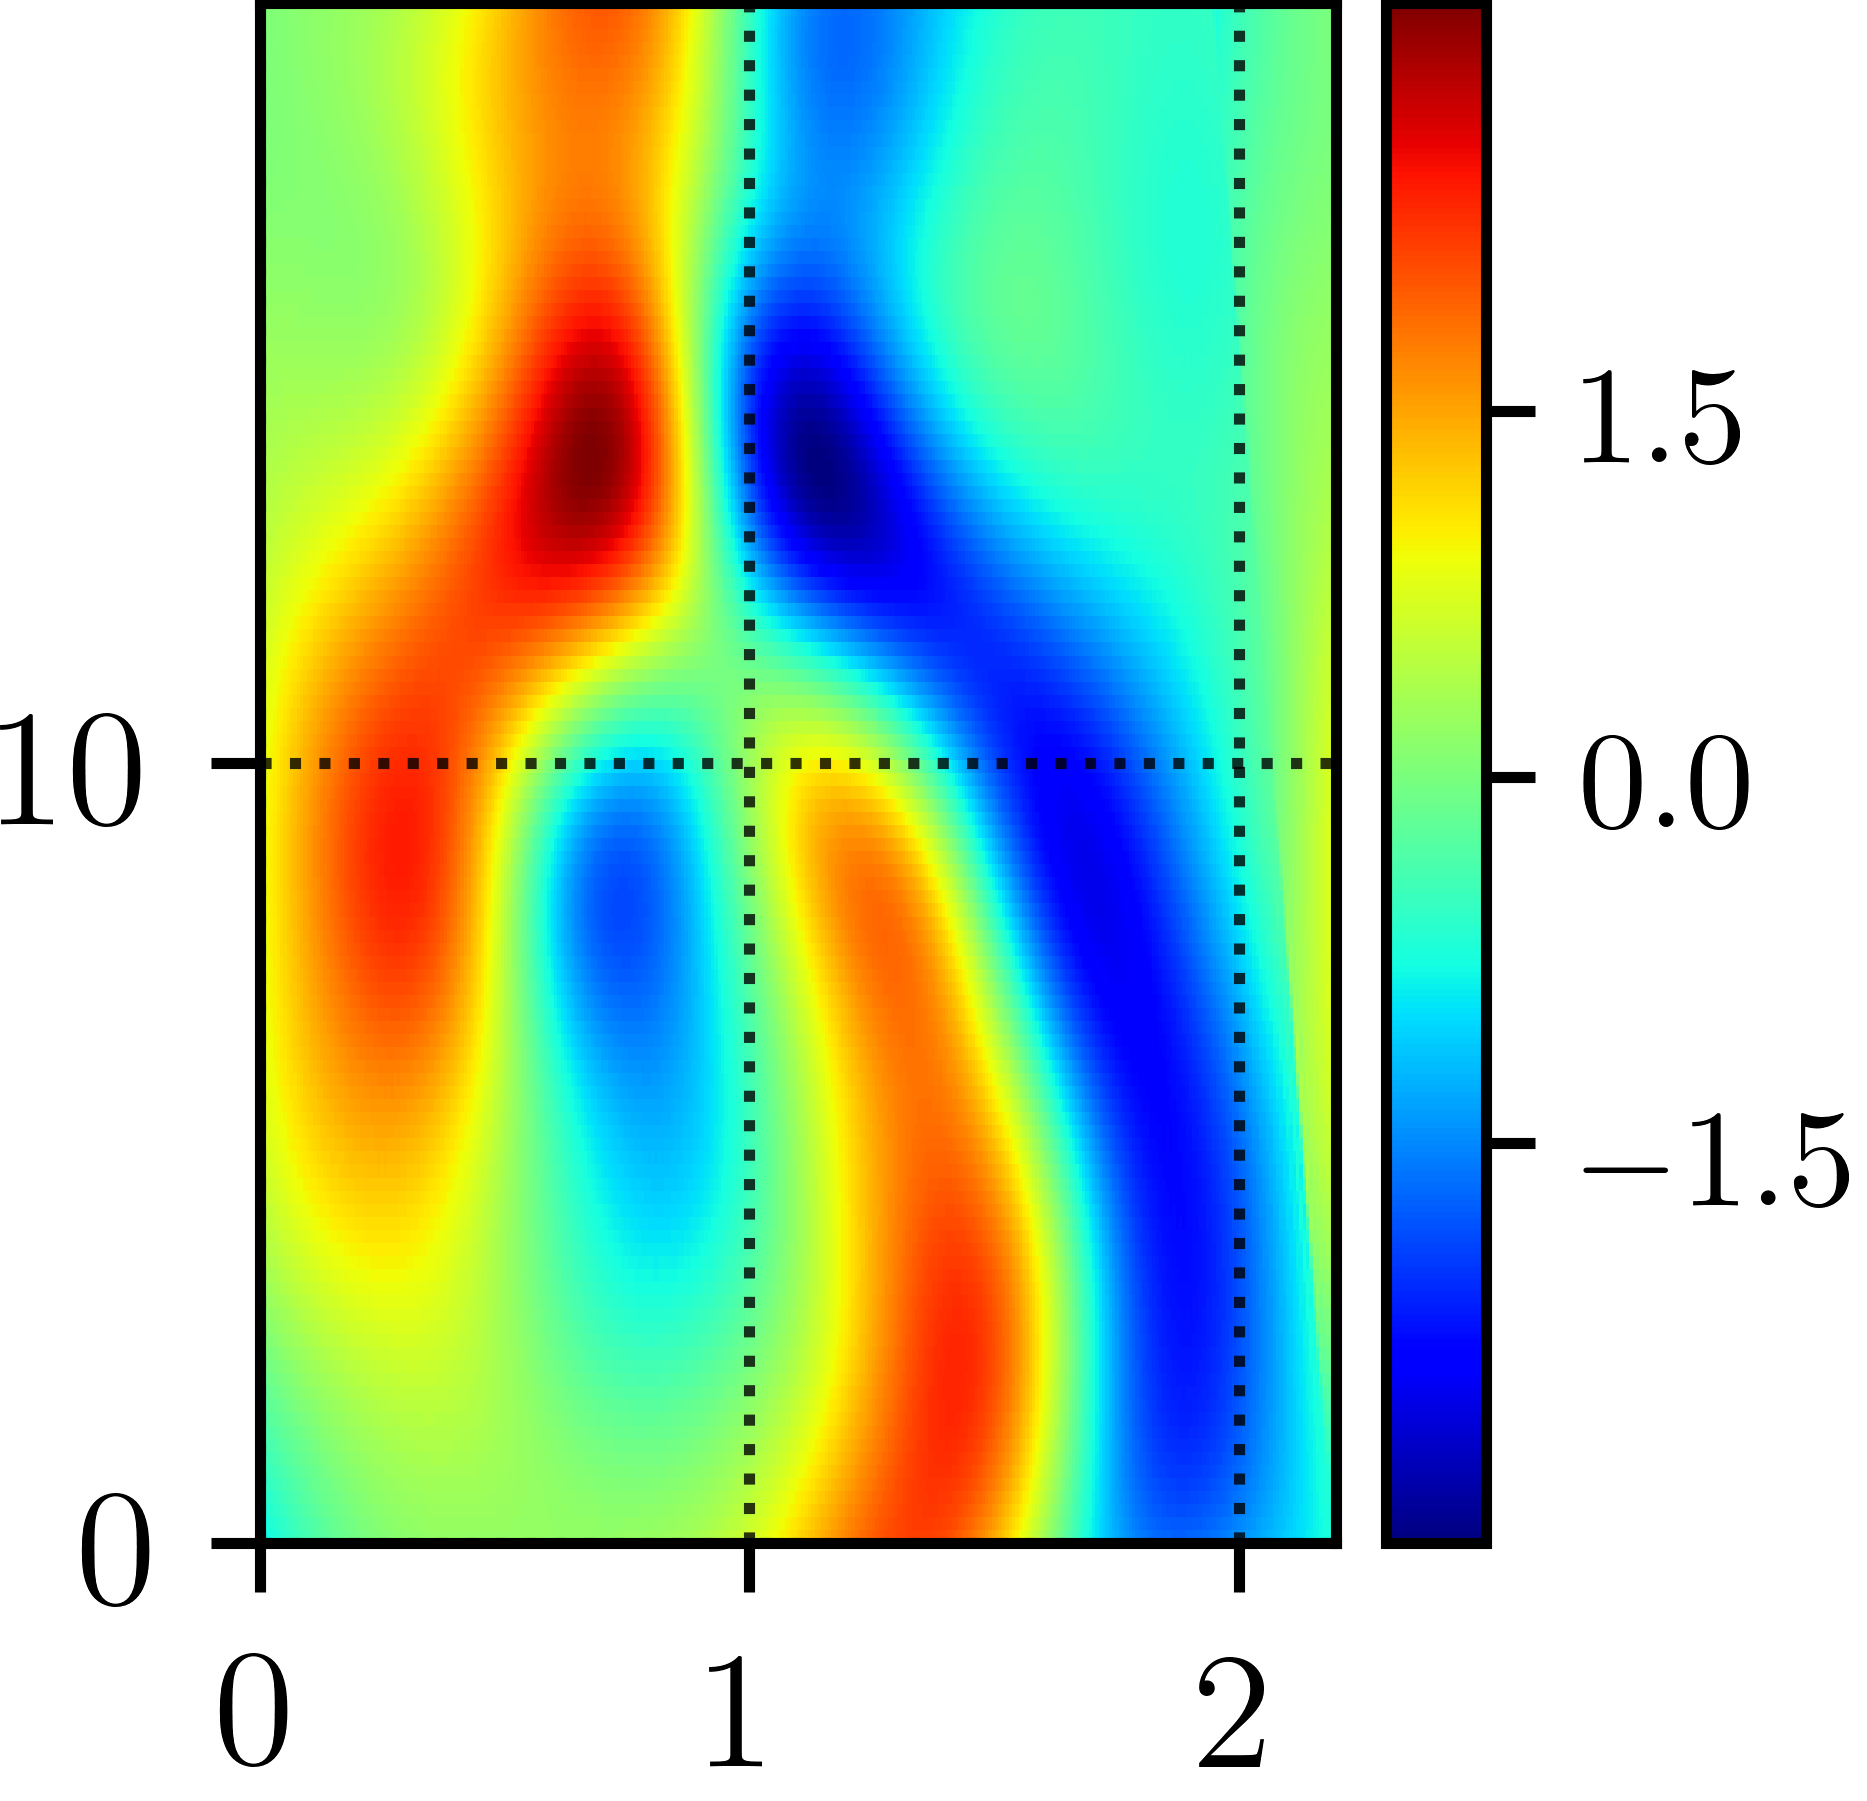
\includegraphics[width=.4\textwidth,height=.1\textheight]{MNG_halfdefecterg}
\end{minipage}
\begin{minipage}[height=.05\textheight]{.3\textwidth}
\centering \small{\texttt{(d)}}\\
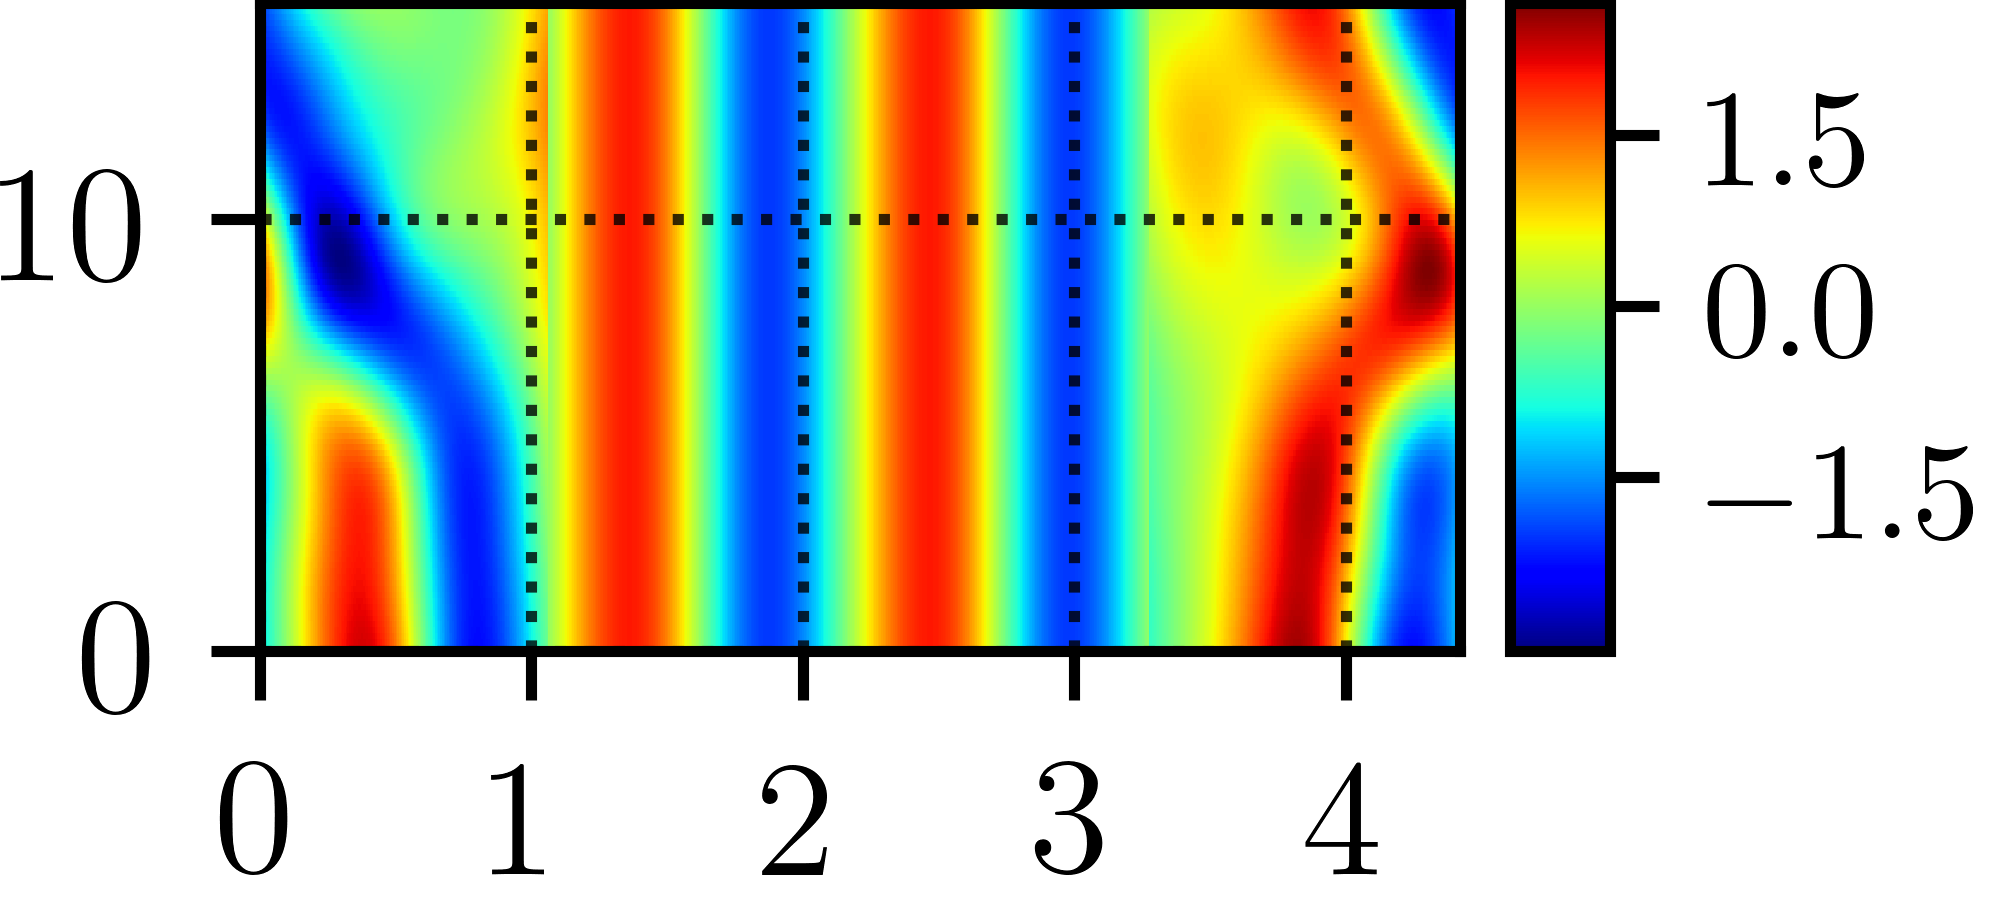
\includegraphics[width=.8\textwidth,height=.1\textheight]{MNG_tiling_subdomain0}
\end{minipage}
\begin{minipage}[height=.05\textheight]{.3\textwidth}
\centering \small{\texttt{(e)}}\\
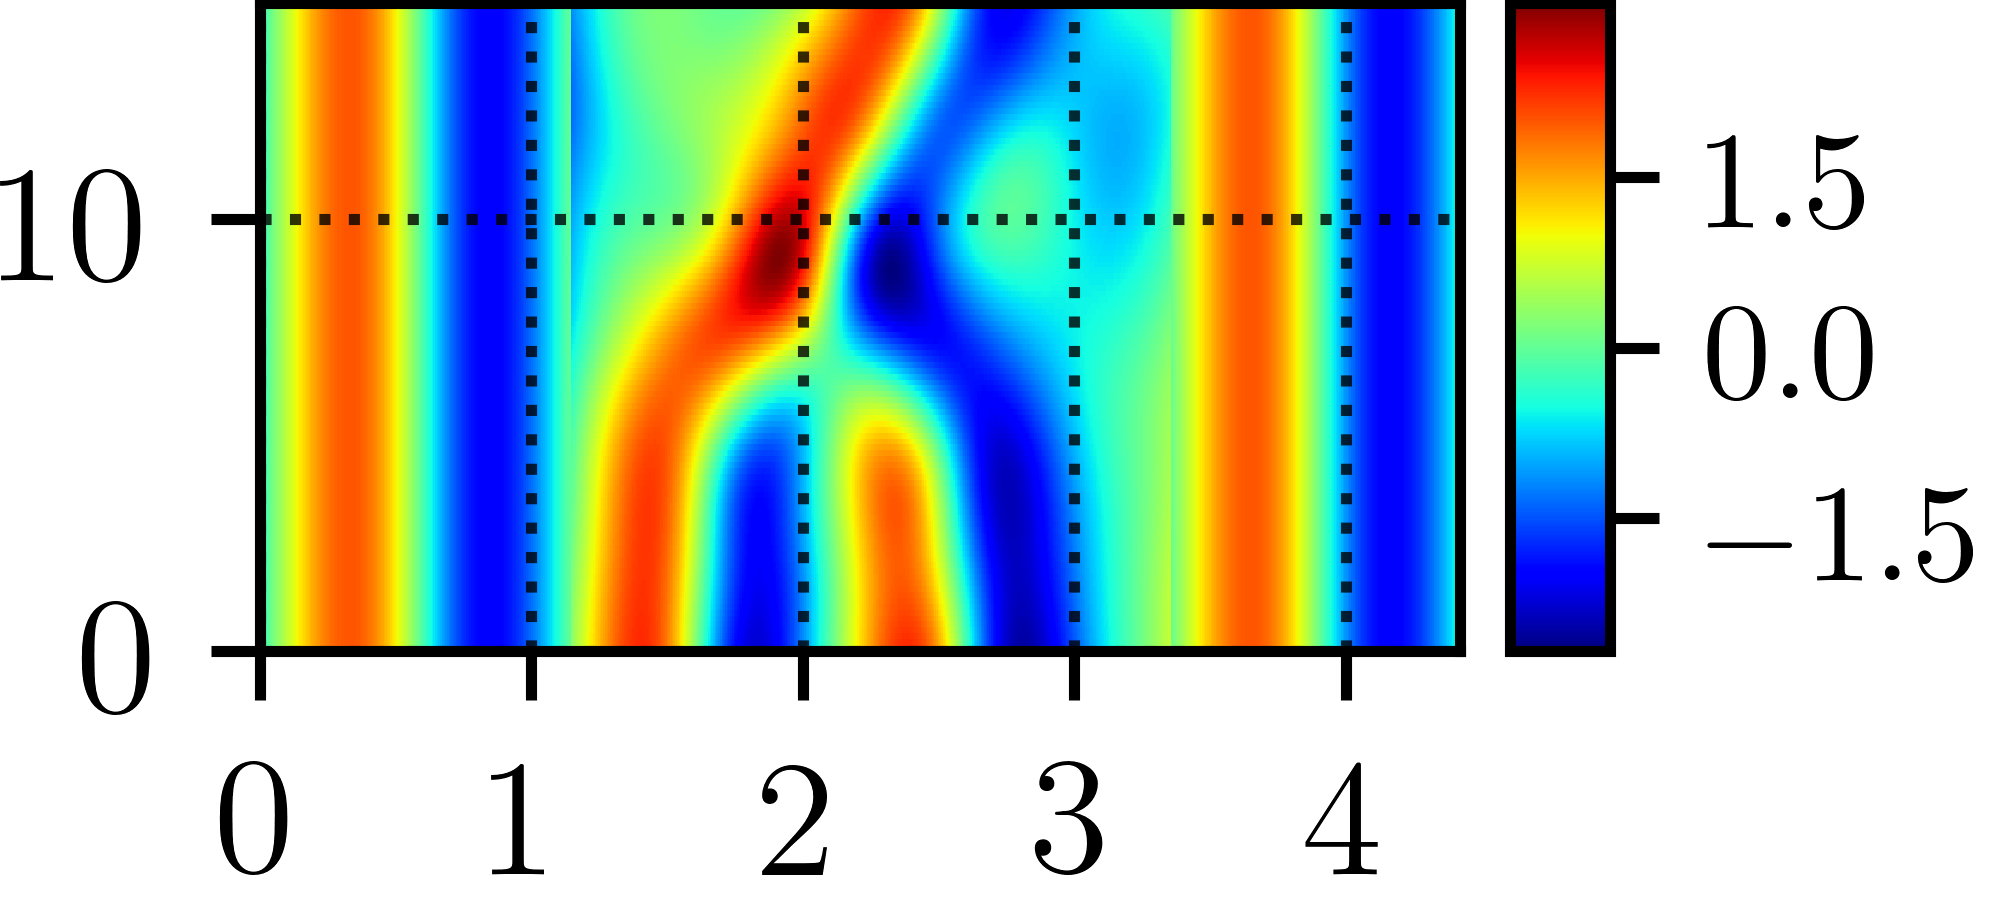
\includegraphics[width=.8\textwidth,height=.1\textheight]{MNG_tiling_subdomain1}
\end{minipage}
\begin{minipage}[height=.05\textheight]{.3\textwidth}
\centering \small{\texttt{(f)}}\\
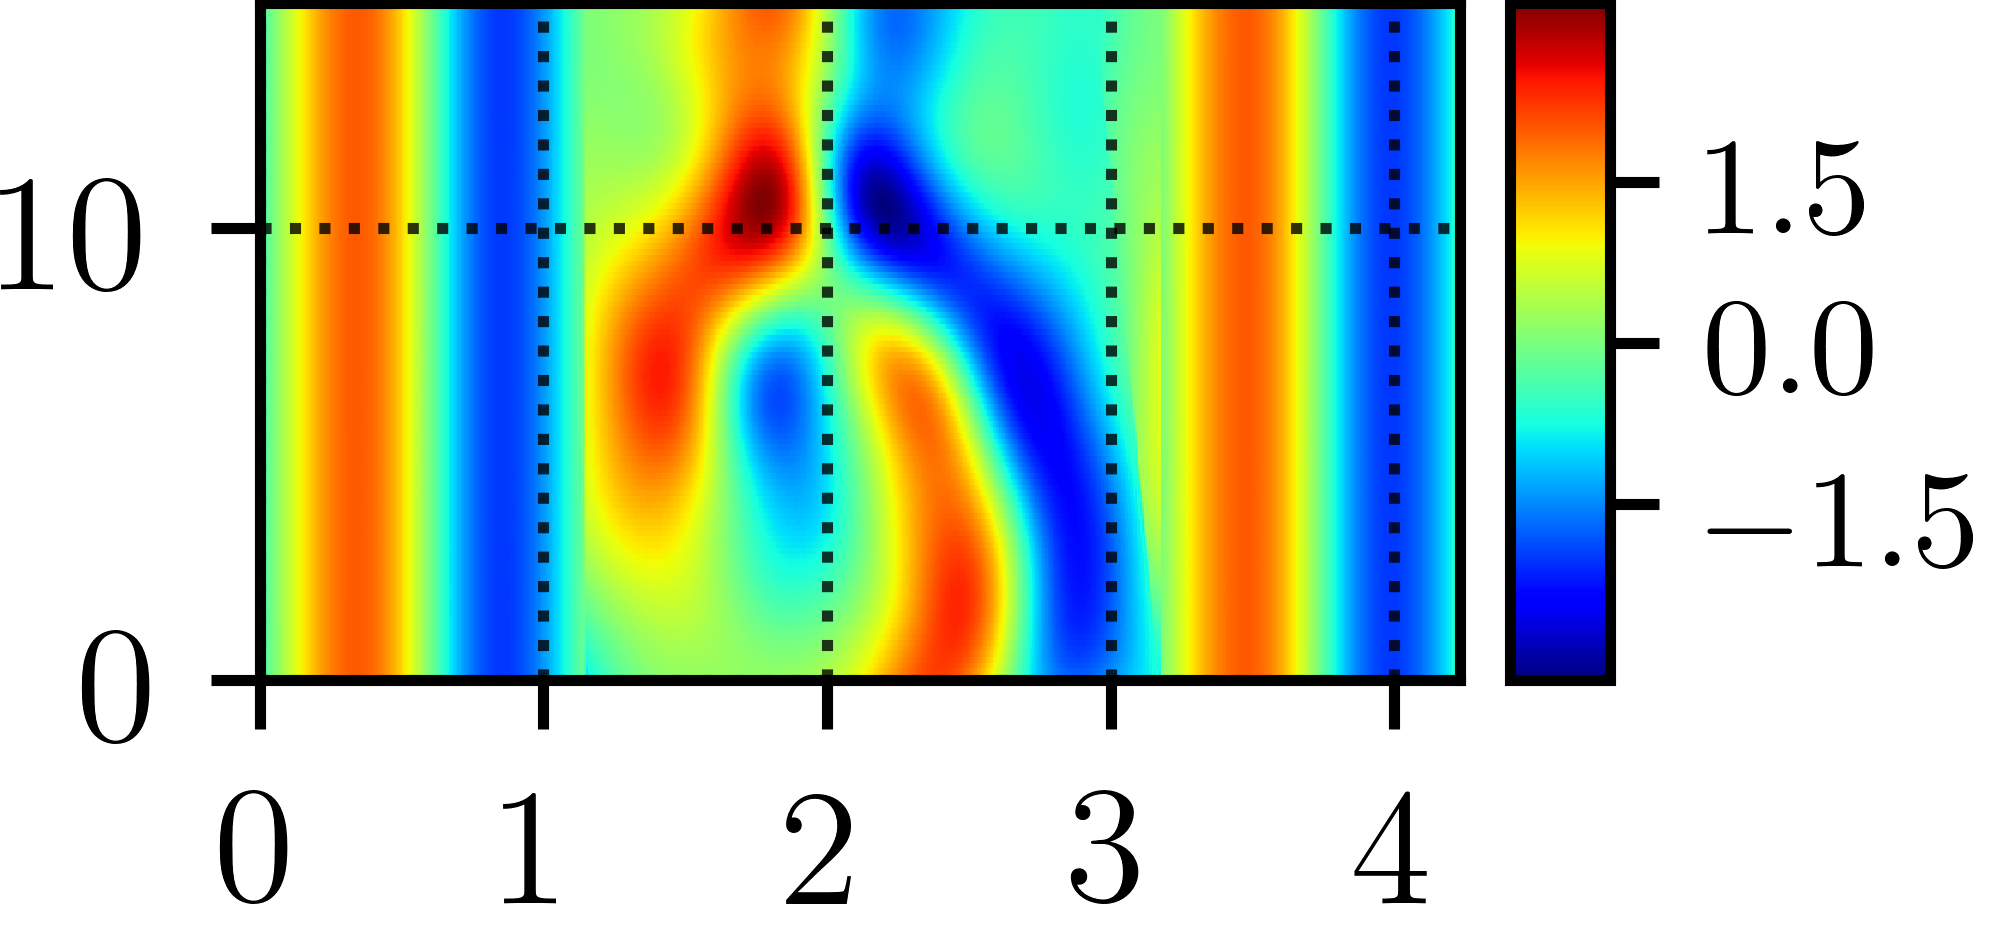
\includegraphics[width=.8\textwidth,height=.1\textheight]{MNG_tiling_subdomain2}
\end{minipage}
\begin{minipage}[height=.1\textheight]{.35\textwidth}
\centering \small{\texttt{(g)}}\\
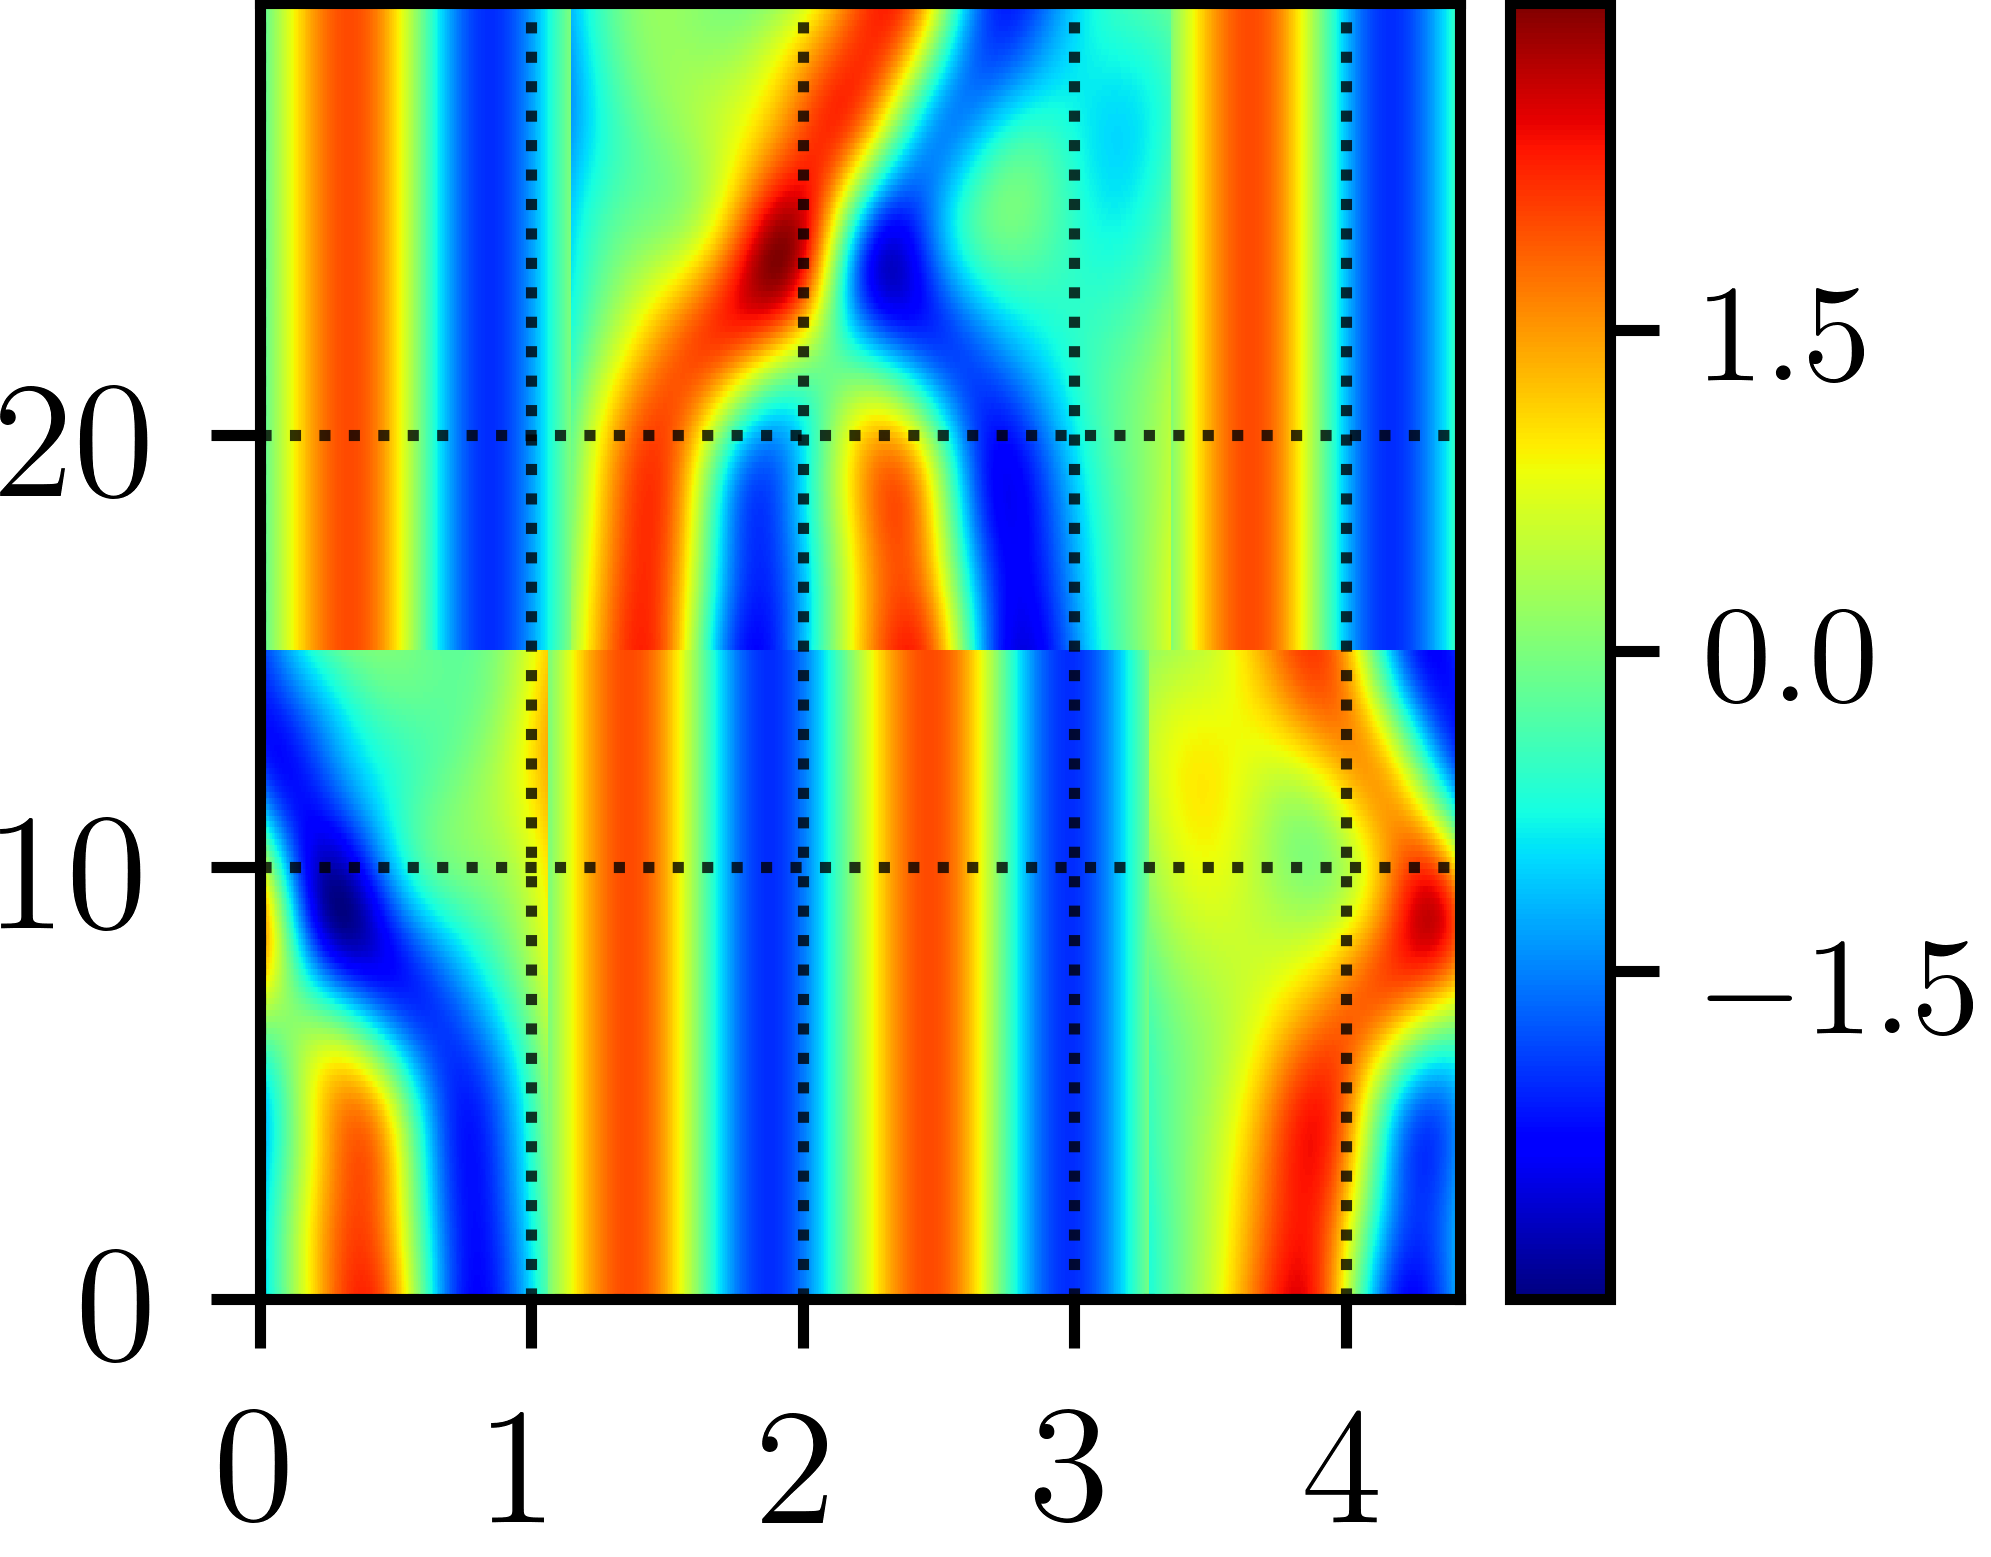
\includegraphics[width=.8\textwidth,height=.28\textheight]{MNG_tiling_twosubdomains}
\end{minipage}
\begin{minipage}[height=.15\textheight]{.3\textwidth}
\centering \small{\texttt{(h)}}\\
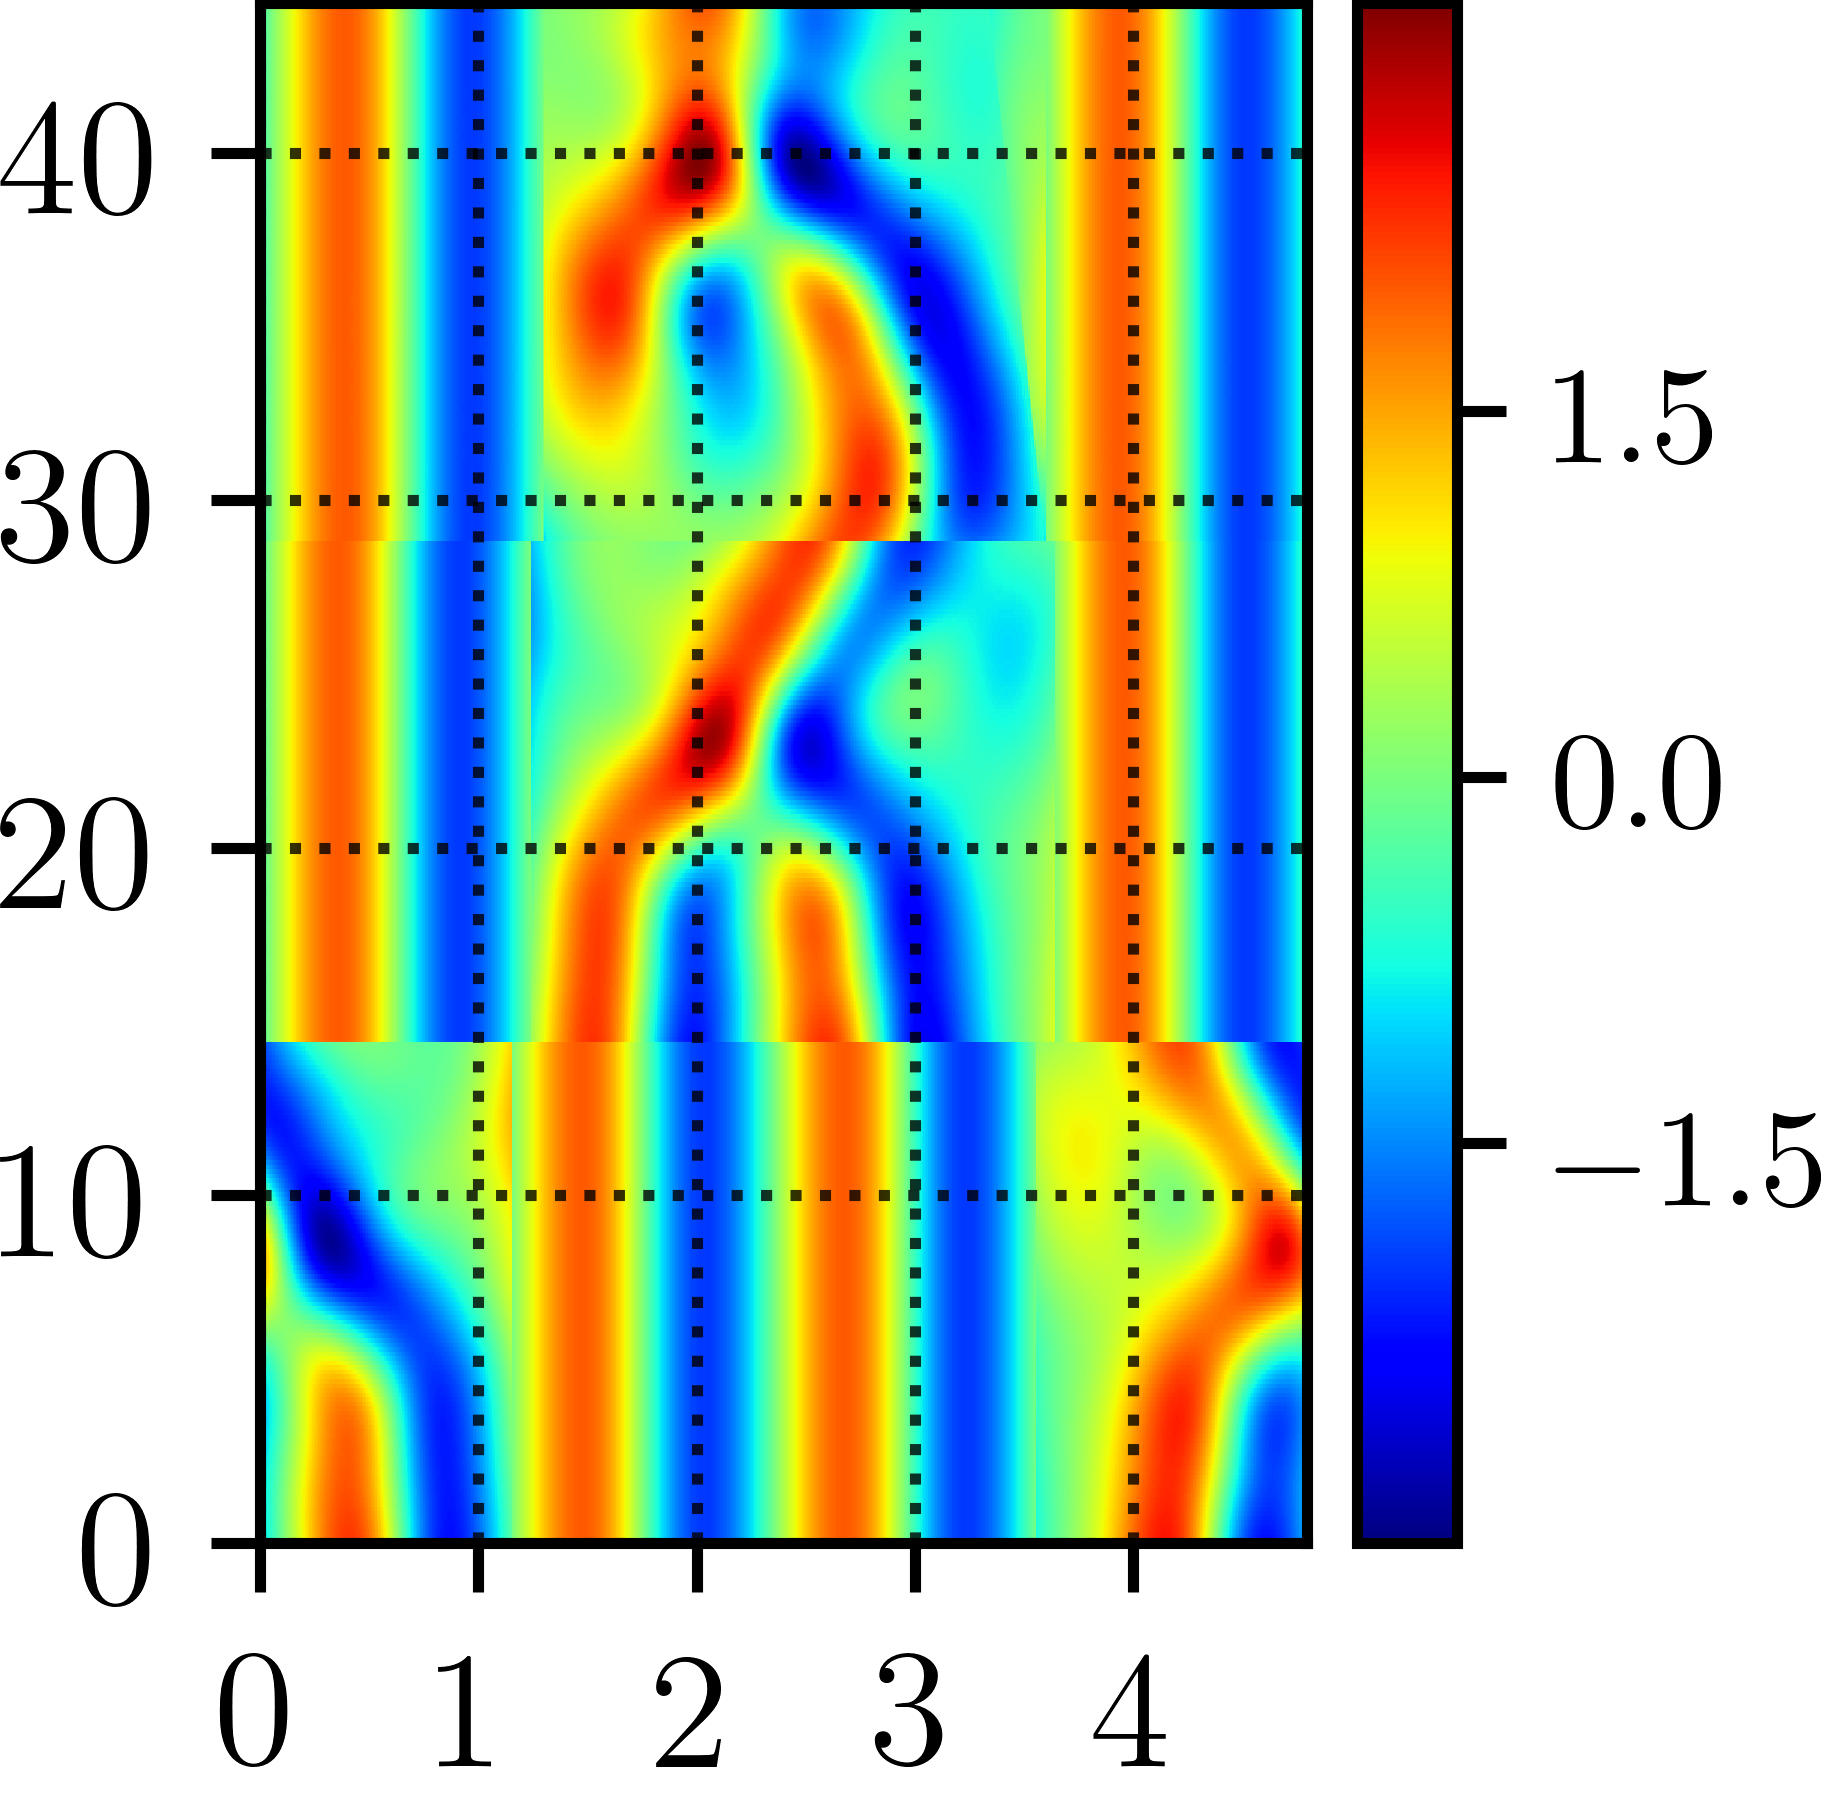
\includegraphics[width=\textwidth,height=.36\textheight]{MNG_tiling_fundamental}
\end{minipage}
\begin{minipage}[height=.15\textheight]{.3\textwidth}
\centering \small{\texttt{(i)}}\\
\includegraphics[width=\textwidth,height=.36\textheight]{MNG_tiling_initial}
\end{minipage}

\caption{ \label{fig:tilingschematic}
Demonstration of how to construct an initial condition corresponding to a specific
\spt\ symbolic block. (a),(b) and (c) together are the set of tiles used for all
other plots in this figure. (d) is a subdomain comprised of two copies of (a) and one copy of (b). (e) is a subdomain comprised of two copies of (a) and one copy of
the reflection of (b). (f) is a subdomain comprised of two copies of (a) and a
single copy of (c). The last row of figures demonstrate how to combine (d),(e),
and (f). (g) is the combination of (d) and (e). (h) is the combination of (d),(e)
and (f) (equivalently, (g) and (f)). Lastly (i) is the smoothed version of (h) which will serve as the initial condition.
}
\end{figure}
We have displayed that it is possible to find small \spt\ \twots\ that
are embedded in larger \twots.
Now we will demonstrate the opposite,
finding larger \twots\ by combining smaller \twots, is also possible in a method we
call ``tiling''. Not only will this provide us with yet another
method to find \twots\ but also it will allow us to investigate
the symbolic dynamics of our \spt\ system.
Specifically, we will investigate the grammar
\rf{AACI,BuBoCvSi14} or set of rules that dictates
which symbolic sequences are admissible or, in other words, which tilings will
be physically realized as \twots. In general, symbolic dynamics may be
arbitrarily complex even in systems as simple as the logistic map\rf{AACI}.
In spite of this, we will attempt to reverse engineer the grammar
by using brute force, no less. This brute force method consists of
finding all admissible tilings. With the inadmissible tiling combinations
we hope to construct a consistent grammar, or at least find an approximate
grammar that can be used as rough guideline.
First, however, a method to create initial conditions from combining
tiles was required.
The crudest way to do so is to numerically
combine them without any preprocessing; this introduces numerical discontinuities
at every conjunction of tiles.
We expend slightly more effort handling these discontinuities
by numerically padding the tiles with a boundary of grid points, all
initialized with a field value of zero. This creates buffer regions between
tiles or ``zero padding'', which aims to smooth the field and
bring it closer to being periodic.
In addition
to this zero padding, we also truncate the \spt\ \Fcs\ for further smoothing.
One downside to this two step method is that it
creates initial conditions with localized \spt\ features;
this is unnatural for the \KSe\ because of its linearly unstable modes.
An alternative would be to approximately solve the boundary value problem
induced by the zero padding, using a Chebyshev polynomial
collocation method, for instance. Because of the non periodic
boundary conditions in this augmented problem,
it may very well be more difficult that our original problem, hence
why we avoid such calculations.

There are many subtleties and details to consider for
the automated tiling method. For instance, the discretization
of each tile needs to be modified so that tiles are combined
with the correct aspect ratios.
In the case of the streak tile this is not very straightforward because
it does not have an intrinsic timescale (other than zero if you would like).
Currently, we make the simple but crude choice which is to say that
the period is not affected by combination with streak tiles. We leave any
error introduced by this assumption to our numerical
optimization procedure. Because we are only creating initial conditions
which are not themselves solutions we are able to be less than perfect.
There are of course many other numerical details but also theoretical details
which would improve this process. Some details that we have
not implemented nor investigated are how
the energetics of the tiles or their local Galilean velocities affect
the tiling procedure. We stated in \refsect{sect:KSsymm} that the
Galilean invariance \refeq{GalInv} is used to set the mean velocity of
the overall front to zero.
For an arbitrary subregion of width $\speriod{1}< \speriod{}$, the
mean velocity is generically $\spaceAver{u}(\zeit)\neq0$. Actually, we
know that as function of $\speriod{}$ the velocity front executes a
random walk,
    \PC{2019-12-06}{make sure that this is explained in the
text elsewhere, then link here to the variance equation
``with variance
$E(\zeit)=\half\spaceAver{u^2}(\zeit)\propto\speriod{}$ by the
extensivity of \KS,''
    }
and hence the range of the color bar in a figure such
as \reffig{f:ks_largeL} has to grow proportionally to
$\sqrt{\speriod{}}$. The variance grows only in the spatial direction, in
the time direction $E(\zeit)\to{E}$.
That implies that in gluing letters $u_j$ of alphabet
\reffig{fig:tiles} into larger patterns, one also has to vary
$\spaceAver{u_j}(\zeit)$ averaged over the tile of width $\speriod{j}$,
in order to glue optimally. In other words, we have to use the Galilean
symmetry group orbit of the letter $u_j$, and slice that group orbit at
$\spaceAver{u_j}(\zeit_0)=0$ for purposes of plotting its representative
in \reffig{fig:tiles}. The tiles \reffig{fig:tiles} were all converged
with under the zero mean velocity condition; locally, subdomains of
the tiling has local Galilean velocities so long as the subdomain is not
a tile (or a tile plus zero padding, as zeroes do not contribute to the integral
\refeq{GalInv}).
In summary there are many different properties that we have not taken
into account and so any results can really only be validated numerically.

We move on to the results and utility of our tiling method.
We begin with a simple tiling example
which iteratively adds the streak tile in the spatial direction
to the merger tile.
The symbolic
blocks \refeq{e-block01},\refeq{e-block001},\refeq{e-block0001}
represent these tilings (in theory).
In all tiling examples that follow, the \twots\
are converged in the full state space; that is,
they have only the trivial subgroup as their isotropy
subgroups.

\beq
\Mm=\left[\begin{array}{c}
0 1
\end{array}\right]
\ee{e-block01}

\beq
\Mm=\left[\begin{array}{c}
0 0 1
\end{array}\right]
\ee{e-block001}

\beq
\Mm=\left[\begin{array}{c}
0 0 0 1
\end{array}\right]
\ee{e-block0001}

As we can see in the collection of \reffig{fig:block01}, \reffig{fig:block001},
\reffig{fig:block0001}. From the \spt\ dimensions of the tiles in \reffig{fig:tiles}
we can see that simple addition would predict that \reffig{fig:block01} should
have spatial domain size approximately equal
to $\speriod{01} \approx \speriod{s}+\speriod{m}=3.09$. The true value
comes out to $\speriod{01}=3.13\cdots$. Likewise, each new streak addition
should approximately modify the spatial domain size in the same way, which
is exactly what occurs, as $\speriod{001}=4.12\cdots$ and
$\speriod{0001}=5.16\cdots$. Note that in each step both $\speriod{}$ and $\period{}$
change by a different amount such that the resulting \twot\ satisfies \refeq{e-ks}.
This is expected as we are allowing both dimensions to change, we are solving
the equations in a least-squares manner, and of course the equations are nonlinear.

\begin{figure}
\begin{minipage}[height=.4\textheight]{.5\textwidth}
\centering \small{\texttt{(a)}}\\
\includegraphics[width=.3\textwidth,height=.15\textheight]{MNG_01_initial}
\end{minipage}
\begin{minipage}[height=.4\textheight]{.5\textwidth}
\centering \small{\texttt{(b)}}\\
\includegraphics[width=.3\textwidth,height=.18\textheight]{MNG_01_final}
\end{minipage}
\caption{ \label{fig:block01}
(a) Initial \spt\ field for the one-by-two symbolic block given by \refeq{e-block01}
(b) \twoT\ resultant from numerically converging (a),
$[\speriod{b},\period{b}]=[3.13\cdots,20.84\cdots]$
}
\end{figure}

\begin{figure}
\begin{minipage}[height=.4\textheight]{.5\textwidth}
\centering \small{\texttt{(a)}}\\
\includegraphics[width=.4\textwidth,height=.15\textheight]{MNG_001_initial}
\end{minipage}
\begin{minipage}[height=.4\textheight]{.5\textwidth}
\centering \small{\texttt{(b)}}\\
\includegraphics[width=.4\textwidth,height=.23\textheight]{MNG_001_final}
\end{minipage}
\caption{ \label{fig:block001}
(a) Initial \spt\ field for the one-by-three symbolic block given by \refeq{e-block001}
(b) \twoT\ resultant from numerically converging (a),
$[\speriod{b},\period{b}]=[4.12\cdots,23.15\cdots ]$.
}
\end{figure}

\begin{figure}
\begin{minipage}[height=.4\textheight]{.45\textwidth}
\centering \small{\texttt{(a)}}\\
\includegraphics[width=.55\textwidth,height=.15\textheight]{MNG_0001_initial}
\end{minipage}
\begin{minipage}[height=.4\textheight]{.45\textwidth}
\centering \small{\texttt{(b)}}\\
\includegraphics[width=.6\textwidth,height=.23\textheight]{MNG_0001_final}
\end{minipage}
\caption{ \label{fig:block0001}
(a) Initial \spt\ field for the one-by-four symbolic block given by \refeq{e-block0001}
(b) \twoT\ resultant from numerically converging (a),
$[\speriod{b},\period{b}]=[5.16\cdots,23.77\cdots]$.
}
\end{figure}

We have established that it is at least possible to find solutions
by our tiling method but we need some way to confirm our results.
First, the converged \twot\ resulting from a symbolic sequence should
be invariant under symmetry transformations of the symbols themselves.
We provide an example of this
in \refeq{e-block012} and \refeq{e-block201}.
The two symbolic blocks in question are spatial rotations
of one another but they
numerically converge to \twots\ which are only approximately
related by the same rotation, as seen in \reffig{fig:block012} and
\reffig{fig:block201}. The reason why the two converged solutions
do not differ only by spatial rotation, as one might
expect, is because the solutions are being found in a least-squares
manner and the initial \spt\ \Fcs\ differ by a phase factor.
This phase difference is sufficient enough to affect the numerical results.
In this manner, the numerical methods and symmetry actions are only
approximately ``conjugate''; in other words, the order technically matters.
Specifically, the discrepancy of the solutions can mainly be explained
by their differing domain sizes. These \spt\ domain sizes are
$[\speriod{b},\period{b}]=[6.36\cdots,24.98\cdots]$ and
$[\speriod{b},\period{b}]=[6.07\cdots,16.58\cdots]$ for \refeq{e-block012}
and \refeq{e-block201} respectively. We expect that numerical continuation
in \spt\ domain size would be able to connect these solutions such
that the results would be the same field up to a symmetry operation. This
belief comes from performing exactly this computation for tiles in \reffig{fig:tilerepeats}.
This idea should of course be applicable to all symmetry related symbolic blocks
but it is technically possible that for a large tiling the phase factor can change
which \twot\ the initial condition converges to. This has not been confirmed not
denied but we offer this possibility as a caution for others.

\beq
\Mm=\left[\begin{array}{c}
0\,1\,2
\end{array}\right]
\ee{e-block012}

\beq
\Mm=\left[\begin{array}{c}
2\,0\,1
\end{array}\right]
\ee{e-block201}


\begin{figure}
\begin{minipage}[height=.4\textheight]{.5\textwidth}
\centering \small{\texttt{(a)}}\\
\includegraphics[width=.6\textwidth,height=.15\textheight]{MNG_012_initial}
\end{minipage}
\begin{minipage}[height=.4\textheight]{.5\textwidth}
\centering \small{\texttt{(b)}}\\
\includegraphics[width=.6\textwidth,height=.25\textheight]{MNG_012_final}
\end{minipage}
\caption{ \label{fig:block012}
(a) Initial \spt\ field for the one-by-three given by \refeq{e-block012}
(b) \twoT\ resultant from numerically converging (a),
$[\speriod{b},\period{b}]=[6.36\cdots,24.98\cdots]$.
}
\end{figure}

\begin{figure}
\begin{minipage}[height=.4\textheight]{.5\textwidth}
\centering \small{\texttt{(a)}}\\
\includegraphics[width=.6\textwidth,height=.15\textheight]{MNG_201_initial}
\end{minipage}
\begin{minipage}[height=.4\textheight]{.5\textwidth}
\centering \small{\texttt{(b)}}\\
\includegraphics[width=.6\textwidth,height=.15\textheight]{MNG_201_final}
\end{minipage}
\caption{ \label{fig:block201}
(a) Initial \spt\ field for the one-by-three symbolic block given by \refeq{e-block201}
(b) \twoT\ resultant from numerically converging (a),
$[\speriod{b},\period{b}]=[6.07\cdots,16.58\cdots]$.
}
\end{figure}

Both examples so far have only considered spatial tiling. The general
case, tiling \spt\ patterns, is a much more appropriate demonstration
of tiling.
To demonstrate this extension,
we create two initial conditions corresponding to
the two-by-two symbolic blocks \refeq{e-block0110}
and \refeq{e-block0210}, as well as a
simple three-by-three symbolic
block example \refeq{e-block000000002}.

\beq
\Mm=\left[\begin{array}{c}
0\,1 \\
1\,0
\end{array}\right]
\ee{e-block0110}

\beq
\Mm=\left[\begin{array}{c}
0\,2 \\
1\,0
\end{array}\right]
\ee{e-block0210}


\beq
\Mm=\left[\begin{array}{c}
0\,0\,0 \\
0\,0\,0 \\
0\,0\,2
\end{array}\right]
\ee{e-block000000002}

All three of these initial conditions converge numerically, as indicated
in the corresponding figures \reffig{fig:block0110},
\reffig{fig:block0210}, \reffig{fig:block000000002}. \refFig{fig:block0110}
converges to a \twot\ closest to what one might expect as the second half
of the orbit (in time) seems to be very close to a reflection of the first
half, a property restricted to shift-reflection invariance. This makes
sense due to the antisymmetric (approximately in the merger tile's case)
nature of the tiles themselves. Meanwhile, it is hard
to distinguish whether \reffig{fig:block000000002} is a quality result or not.
By construction of the initial condition there are three wavelengths
represented by the first two ``rows'' of the symbolic block, but four
wavelengths in the last row. The converged \twot, however, seems to
converge to a solution that has three well defined (amplitude) wavelengths
at any given time. This result appeals to our knowledge of the physical
scales of the \KSe\ as the initial domain size is closer to three multiples
of the most unstable wavelength than four.

\begin{figure}
\begin{minipage}[height=.4\textheight]{.45\textwidth}
\centering \small{\texttt{(a)}}\\
\includegraphics[width=.5\textwidth,height=.3\textheight]{MNG_01_10_initial}
\end{minipage}
\begin{minipage}[height=.4\textheight]{.45\textwidth}
\centering \small{\texttt{(b)}}\\
\includegraphics[width=.5\textwidth,height=.4\textheight]{MNG_01_10_final}
\end{minipage}
\caption{ \label{fig:block0110}
(a) Initial \spt\ field for the two-by-two symbolic block given by \refeq{e-block0110}
(b) \twoT\ resultant from numerically converging (a),
$[\speriod{b},\period{b}]=[3.64\cdots,45.26\cdots]$.
}
\end{figure}

\begin{figure}
\begin{minipage}[height=.4\textheight]{.45\textwidth}
\centering \small{\texttt{(a)}}\\
\includegraphics[width=.5\textwidth,height=.3\textheight]{MNG_02_10_initial}
\end{minipage}
\begin{minipage}[height=.4\textheight]{.45\textwidth}
\centering \small{\texttt{(b)}}\\
\includegraphics[width=.5\textwidth,height=.4\textheight]{MNG_02_10_final}
\end{minipage}
\caption{ \label{fig:block0210}
(a) Initial \spt\ field for the two-by-two symbolic block given by \refeq{e-block0210}
(b) \twoT\ resultant from numerically converging (a),
$[\speriod{b},\period{b}]=[3.19\cdots,45.81\cdots]$.
}
\end{figure}

\begin{figure}
\begin{minipage}[height=.4\textheight]{.45\textwidth}
\centering \small{\texttt{(a)}}\\
\includegraphics[width=.5\textwidth,height=.15\textheight]{MNG_000_000_002_initial}
\end{minipage}
\begin{minipage}[height=.4\textheight]{.45\textwidth}
\centering \small{\texttt{(b)}}\\
\includegraphics[width=.5\textwidth,height=.15\textheight]{MNG_000_000_002_final}
\end{minipage}
\caption{ \label{fig:block000000002}
(a) Initial \spt\ field for the three-by-three symbolic block given by \refeq{e-block000000002}.
(b) \twoT\ resultant from numerically converging (a),
$[\speriod{b},\period{b}]=[3.89\cdots,19.22\cdots]$.
}
\end{figure}

In light of these results,
recall that our original goal was to explain the \spt\ symbolic dynamics
by enumerating all admissible tilings; so far, the results
have been good numerically but poor in regards to the symbolic dynamics.
Most of the tilings converge numerically but it is not
evident that they always converge to the targeted
symbolic block. We have only been
able to tell by manually inspection of the features
of each converged block. The features in the converged \twot\
should of course match the symbolic block, at least up to continuous
deformations.
If \twots\ shadow too many or too few \twots, then that
initial condition has likely converged to
a different symbolic block.
This possibility is unsettling in terms of the development of our
symbolic dynamics. Errant convergence only serves to misinform us
regarding the grammar of the symbolic dynamics.
How can we determine if a converged \twot\
is indeed a representation of a specific symbolic sequence or not?
For validation of our results we seek a numerical method that
can detect tiles embedded in large \twots.
This method also needs to account for continuous families of tile deformations;
therefore, it seems natural to search for a method which searches for
specific features.

We can postulate some methods but we have not created a method
that can automatically validate converged symbolic \twots. For instance,
we can use an image processing technique, ``feature detection''.
Image ``features'' are very loosely defined and they can be as general
as corners or edges; of course we need to tune this to
detect signatures of different tiles instead. The primary
property of these features is that they can be detected
even after different transformations of the image such as
affine transformations. This of course is good as the signatures
of our tiles manifest differently for each continuous tile
deformation.
First, we begin by representing the \twot\ as a grey scale
images. Once a gray scale image is produced, we utilize
numerical methods from the Python package \texttt{scikit-image} for
the feature detection.
The results are quite striking in regards to how tiles are represented by specific
shapes even after such a large amount of data reduction.
In this representation streaks still manifest as streaks. Creations of streaks, however,
is represented by an upwards facing pitchfork. Annihilation of streaks (merger tile) is
represented by downward facing pitchforks (in this case there
it is possible to see ``imperfect pitchforks'' like from bifurcation theory).
There is a thick wishbone type shape
which represents a gap and a ring like structure on the left side on
the domain which appears to represent either a hook (member of the
merger tile family).
Using these shapes as indicators we believe that \reffig{f:MNGblockfeatures}(a) is \textit{not} a
representation of the symbolic sequence $1012$ as previously believed; determined
by inspecting the \spt\ ordering of these features.
The features that are detected seems
to be heavily dependent on the parameter values input into the numerical method.
The ideal case for us is to only detect non-streak features. This is desirable
because if we find locations of all gap and merger tiles, the remainder of the \twot\
should be covered by streaks if the alphabet is trinary. The problem with this is that
the feature detection picks up creation of streaks which isn't useful.
Tuning the different parameters of the \texttt{ORB} feature detection scheme
from \texttt{scikit-image} package produces a set of data points
which cluster around the desired features. by analyzing the pixel intensities
of the image. We apply this to two different examples; the converged \twot\
from a tiling and a ergodic trajectory segment with large \spt\ extent. The first
example is to attempt to validate the symbolic representation we claim, the second
it to see how this scheme holds up when the features are small relative to the image.


\begin{figure}[t]
\begin{minipage}[height=.30\textheight]{.30\textwidth}
\centering
\includegraphics[width=1.0\textwidth]{MNG_block}
\\ \small{\texttt{(a)}}
\end{minipage}
\begin{minipage}[height=.30\textheight]{.30\textwidth}
\centering
\includegraphics[width=1.0\textwidth]{MNG_blockfeatures1}
\\ \small{\texttt{(b)}}
\end{minipage}
\begin{minipage}[height=.30\textheight]{.30\textwidth}
\centering
\includegraphics[width=1.0\textwidth]{MNG_blockfeatures2}
\\ \small{\texttt{(c)}}
\end{minipage}
\caption{\label{f:MNGblockfeatures}
(a) \twoT\ converged in full state space purported to be
symbolic block $1012$ (spatial sequence)
(b),(c) are two separate attempts at ``feature detection'' using
the ``ORB'' numerical routine that is part of \texttt{scikit-image}
}
\end{figure}

\begin{figure}[t]
\begin{minipage}[height=.80\textheight]{.80\textwidth}
\centering
\includegraphics[width=1.0\textwidth]{MNG_uu500b500}
\\ \small{\texttt{(a)}}
\end{minipage}
\begin{minipage}[height=.80\textheight]{.80\textwidth}
\centering
\includegraphics[width=1.0\textwidth]{MNG_largefeatures}
\\ \small{\texttt{(b)}}
\end{minipage}
\caption{\label{f:MNGlargeLfeatures}
(a)Segment of ergodic trajectory produced by time integration
at defined on $[\speriod{},\period{}]=[79.57\cdots,500\cdots]$
(b The result of passing a modified gray scale image of (a) to
the ``ORB'' feature detection
numerical routine that is part of \texttt{scikit-image}
}
\end{figure}

While the accuracy of our symbolic dynamics is
still suspect, it is worth repeating that
we have formulated multiple techniques for
finding \twots. These include
finding large \twots\ by combining small \twots, finding
small \twots\ embedded in large \twots, and
numerical continuation of \twots. These methods work
in tandem with one another; giving
us the ability to search for nearly any sized \twot\ using
previously acquired data. The flexibility and agility
gained from the combination of these methods is substantial
and it allows for a targeted search for \twots.
This flexibility can help us overcome some problems which
are currently present in numerical studies of fluid flow.
Once such example is the wide variety of parameter values
and geometries (boundary conditions) studied
in the world of fluid dynamics which makes comparison
between {\po}s in different flows difficult. If connections
between geometries can be made then obviously direct comparisons
between {\po}s could be made by also the
specific effect of geometry could be more easily targeted.

In any fluid dynamics research one of the most critical
pieces of information is the value of the Reynolds number.
Its importance cannot be understated as this single parameter
dictates entire regimes of fluid behavior; unfortunately its value
varies wildly depending on the geometry and phenomena being studied.
For instance, in computational studies of plane Couette flow, $Re=400$
is a common value\rf{HaKiWa95,W03,Visw07b}. For experimentalists,
the Reynolds number is on the order of thousands in small
scale experiments\rf{DGE00} to tens, even hundreds, of thousands in large scale
experiments\rf{Kendall75}.
Continuation of solutions from one Reynolds number
to another is already performed in dynamical
systems calculations\rf{WFSBC15} but much like the
initial value problem it can be very sensitive to perturbations;
we appeal again to \spt\ techniques. The difference becomes
apparent when attempting to perform numerical continuation of
the spatial domain size.
In the numerical studies of
plane Couette flow\rf{HaKiWa95,W03,Visw07b} there have
been differing choices as to the size of the computational domain.
In this case the qualitative effect isn't drastic because all three
domain sizes are comparatively small. However, quantitative comparisons
and reproduction of results becomes difficult.
One could technically include spatial domain size as a variable in
the dynamical system formulation but we posit that the ill conditioning of
changing the domain size in combination with the exponential instability
of the dynamics will make this a fruitless endeavor.
As we have seen shown it is not only possible for us to
numerically continue \twots\ with respect to domain size but
keep domain size as a variable; we have seen neither of these
techniques in the literature.

A possible objection to these methods is that there is no
real point in varying the domain size as if there was
a desire to study a specific domain size, then one would do just that.
The problem is that as domain size increases it becomes harder
and harder to simply find {\po}s. Therefore, the more we can
leverage already known data the less we waste computational time.
One of the more compelling arguments is by far in favor
of numerical continuation in spatial domain size is the ability
to match changes in experimental setups for whatever reason;
perhaps more precise measurements of the geometry were made,
or perhaps there was a systematic reason why the
setup needs to be changed. Essentially, numerical continuation
and the ability to change the domain size allows for
the tuning of numerical data to match experimental data.
The limits of
continuation in spatial domain size are unknown but
we do know it depends on the specific \twot\ being continued.
This method likely won't be able to doubling the spatial domain size,
but for smaller changes it seems useful.

In addition to tiling; combining \spt\ tiles to find larger \twots,
we can also glue larger \twots\ together to find yet larger \twots.
Although quite similar, we make the distinction between the two
methods because tiling has a symbolic dynamic motivation while gluing
does not.
